%% Beginning of file 'sample62.tex'
%%
%% Modified 2018 January
%%
%% This is a sample manuscript marked up using the
%% AASTeX v6.2 LaTeX 2e macros.
%%
%% AASTeX is now based on Alexey Vikhlinin's emulateapj.cls 
%% (Copyright 2000-2015).  See the classfile for details.
%% AASTeX requires revtex4-1.cls (http://publish.aps.org/revtex4/) and
%% other external packages (laTexsym, graphicx, amssymb, longtable, and epsf).
%% All of these external packages should already be present in the modern TeX 
%% distributions.  If not they can also be obtained at www.ctan.org.
 
%% The first piece of markup in an AASTeX v6.x document is the \documentclass
%% command. LaTeX will ignore any data that comes before this command. The 
%% documentclass can take an optional argument to modify the output style.
%% The command below calls the preprint style  which will produce a tightly 
%% typeset, one-column, single-spaced document.  It is the default and thus
%% does not need to be explicitly stated.
%%
%%
%% using aastex version 6.2
%\documentclass[twocolumn]{aastex62}
\documentclass[twocolumn, linenumbers]{aastex62}
%% The default is a single spaced, 10 point font, single spaced article.
% There are 5 other style options available via an optional argument. They
%% can be envoked like this:
%%
%% \documentclass[argument]{aastex62}
%% 
%% where the layout options are:
%%
%%  twocolumn   : two text columns, 10 point font, single spaced article.
%%                This is the most compact and represent the final published
%%                derived PDF copy of the accepted manuscript from the publisher
%%  manuscript  : one text column, 12 point font, double spaced article.
%%  preprint    : one text column, 12 point font, single spaced article.  
%%  preprint2   : two text columns, 12 point font, single spaced article.
%%  modern      : a stylish, single text column, 12 point font, article with
%% 		  wider left and right margins. This uses the Daniel
%% 		  Foreman-Mackey and David Hogg design.
%%  RNAAS       : Preferred style for Research Notes which are by design 
%%                lacking an abstract and brief. DO NOT use \begin{abstract}
%%                and \end{abstract} with this style.
%%
%% Note that you can submit to the AAS Journals in any of these 6 styles.
%%
%% There are other optional arguments one can envoke to allow other stylistic
%% actions. The available options are:
%%
%%  astrosymb    : Loads Astrosymb font and define \astrocommands. 
%%  tighten      : Makes baselineskip slightly smaller, only works with 
%%                 the twocolumn substyle.
%%  times        : uses times font instead of the default
%%  linenumbers  : turn on lineno package.
%%  trackchanges : required to see the revision mark up and print its output
%%  longauthor   : Do not use the more compressed footnote style (default) for 
%%                 the author/collaboration/affiliations. Instead print all
%%                 affiliation information after each name. Creates a much
%%                 long author list but may be desirable for short author papers
%%
%% these can be used in any combination, e.g.
%%
%% \documentclass[twocolumn,linenumbers,trackchanges]{aastex62}
%%
%% AASTeX v6.* now includes \hyperref support. While we have built in specific
%% defaults into the classfile you can manually override them with the
%% \hypersetup command. For example,
%%
%%\hypersetup{linkcolor=red,citecolor=green,filecolor=cyan,urlcolor=magenta}
%%
%% will change the color of the internal links to red, the links to the
%% bibliography to green, the file links to cyan, and the external links to
%% magenta. Additional information on \hyperref options can be found here:
%% https://www.tug.org/applications/hyperref/manual.html#x1-1.0003
%%
%% If you want to create your own macros, you can do so
%% using \newcommand. Your macros should appear before
%% the \begin{document} command.
%%
\newcommand{\vdag}{(v)^\dagger}
\newcommand\aastex{AAS\TeX}
\newcommand\latex{La\TeX}

%\renewcommand{\footnote}{\textit{\alph{footnote}}}
%\renewcommand{\thefootnote}{\alph{footnote}}

\usepackage{comment}
\usepackage{longtable}
\usepackage{ltablex}
%\usepackage{tabularx}
%\usepackage{xltabular}

\usepackage{mathrsfs}
\usepackage{courier}

\usepackage{threeparttable}
%\usepackage{lscape}
\usepackage{autobreak}
%\usepackage{lscape}
%\usepackage{subfig}
%% Reintroduced the \received and \accepted commands from AASTeX v5.2

%---------------------------------
% You should uncomment out this when you publish.
%%%%%%%\received{January 1, 2018}
%%%%%%%\revised{January 7, 2018}
%%%%%%%\accepted{\today}

%----------------------------------

%% Command to document which AAS Journal the manuscript was submitted to.
%% Adds "Submitted to " the arguement.
\submitjournal{ApJ}

%% Mark up commands to limit the number of authors on the front page.
%% Note that in AASTeX v6.2 a \collaboration call (see below) counts as
%% an author in this case.
%
%\AuthorCollaborationLimit=3
%
%% Will only show Schwarz, Muench and "the AAS Journals Data Scientist 
%% collaboration" on the front page of this example manuscript.
%%
%% Note that all of the author will be shown in the published article.
%% This feature is meant to be used prior to acceptance to make the
%% front end of a long author article more manageable. Please do not use
%% this functionality for manuscripts with less than 20 authors. Conversely,
%% please do use this when the number of authors exceeds 40.
%%
%% Use \allauthors at the manuscript end to show the full author list.
%% This command should only be used with \AuthorCollaborationLimit is used.

%% The following command can be used to set the latex table counters.  It
%% is needed in this document because it uses a mix of latex tabular and
%% AASTeX deluxetables.  In general it should not be needed.
%\setcounter{table}{1}

%%%%%%%%%%%%%%%%%%%%%%%%%%%%%%%%%%%%%%%%%%%%%%%%%%%%%%%%%%%%%%%%%%%%%%%%%%%%%%%%
%%
%% The following section outlines numerous optional output that
%% can be displayed in the front matter or as running meta-data.
%%
%% If you wish, you may supply running head information, although
%% this information may be modified by the editorial offices.
\shorttitle{}
\shortauthors{}
%%
%% You can add a light gray and diagonal water-mark to the first page 
%% with this command:
% \watermark{text}
%% where "text", e.g. DRAFT, is the text to appear.  If the text is 
%% long you can control the water-mark size with:
%  \setwatermarkfontsize{dimension}
%% where dimension is any recognized LaTeX dimension, e.g. pt, in, etc.
%%
%%%%%%%%%%%%%%%%%%%%%%%%%%%%%%%%%%%%%%%%%%%%%%%%%%%%%%%%%%%%%%%%%%%%%%%%%%%%%%%%

%% This is the end of the preamble.  Indicate the beginning of the
%% manuscript itself with \begin{document}.

\begin{document}
\title{Are stripped envelope supernovae really deficient in $^{56}$Ni?}

%\renewcommand{\thefootnote}{\alph{footnote}}

%% LaTeX will automatically break titles if they run longer than
%% one line. However, you may use \\ to force a line break if
%% you desire. In v6.2 you can include a footnote in the title.

%% A significant change from earlier AASTEX versions is in the structure for 
%% calling author and affilations. The change was necessary to implement 
%% autoindexing of affilations which prior was a manual process that could 
%% easily be tedious in large author manuscripts.
%%
%% The \author command is the same as before except it now takes an optional
%% arguement which is the 16 digit ORCID. The syntax is:
%% \author[xxxx-xxxx-xxxx-xxxx]{Author Name}
%%
%% This will hyperlink the author name to the author's ORCID page. Note that
%% during compilation, LaTeX will do some limited checking of the format of
%% the ID to make sure it is valid.
%%
%% Use \affiliation for affiliation information. The old \affil is now aliased
%% to \affiliation. AASTeX v6.2 will automatically index these in the header.
%% When a duplicate is found its index will be the same as its previous entry.
%%
%% Note that \altaffilmark and \altaffiltext have been removed and thus 
%% can not be used to document secondary affiliations. If they are used latex
%% will issue a specific error message and quit. Please use multiple 
%% \affiliation calls for to document more than one affiliation.
%%
%% The new \altaffiliation can be used to indicate some secondary information
%% such as fellowships. This command produces a non-numeric footnote that is
%% set away from the numeric \affiliation footnotes.  NOTE that if an
%% \altaffiliation command is used it must come BEFORE the \affiliation call,
%% right after the \author command, in order to place the footnotes in
%% the proper location.
%%
%% Use \email to set provide email addresses. Each \email will appear on its
%% own line so you can put multiple email address in one \email call. A new
%% \correspondingauthor command is available in V6.2 to identify the
%% corresponding author of the manuscript. It is the author's responsibility
%% to make sure this name is also in the author list.
%%
%% While authors can be grouped inside the same \author and \affiliation
%% commands it is better to have a single author for each. This allows for
%% one to exploit all the new benefits and should make book-keeping easier.
%%
%% If done correctly the peer review system will be able to
%% automatically put the author and affiliation information from the manuscript
%% and save the corresponding author the trouble of entering it by hand.

%1.19167075
%1.19166270
%1.19163



\correspondingauthor{Ryoma Ouchi}
\email{ouchi@kusastro.kyoto-u.ac.jp}
%\affiliation{Department of Astronomy, Kyoto UNiversity, Kitashirakawa-Oiwake-cho, Sakyo-ku, Kyoto 606-8502, Japan}
%\author[0000-0002-0786-7307]{Greg J. Schwarz}
%\affil{American Astronomical Society \\
%2000 Florida Ave., NW, Suite 300 \\
%Washington, DC 20009-1231, USA}
\author{Ryoma Ouchi}

\author{Keiichi Maeda}

\affiliation{Department of Astronomy, Kyoto University, Kitashirakawa-Oiwake-cho, Sakyo-ku, Kyoto 606-8502, Japan}

\author{Joseph P. Anderson}
\affiliation{European Southern Observatory, Alonso de Córdova 3107, Casilla 19, Santiago, Chile}

\author{Ryo Sawada}
\affiliation{Department of Astrophysics and Atmospheric Sciences, Faculty of Science, Kyoto
Sangyo University, Motoyama, Kamigamo, Kita-ku, Kyoto 603-8555, Japan}



%% Note that the \and command from previous versions of AASTeX is now
%% depreciated in this version as it is no longer necessary. AASTeX 
%% automatically takes care of all commas and "and"s between authors names.

%% AASTeX 6.2 has the new \collaboration and \nocollaboration commands to
%% provide the collaboration status of a group of authors. These commands 
%% can be used either before or after the list of corresponding authors. The
%% argument for \collaboration is the collaboration identifier. Authors are
%% encouraged to surround collaboration identifiers with ()s. The 
%% \nocollaboration command takes no argument and exists to indicate that
%% the nearby authors are not part of surrounding collaborations.

%% Mark off the abstract in the ``abstract'' environment.
\begin{abstract}
The nuclear decay of $^{56}$Ni is one of the most important power sources of supernovae (SNe). Recent works have indicated that the $^{56}$Ni masses estimated for Stripped Envelope SNe (SESNe) are systematically higher than those estimated for SNe II. Although this may suggest a distinct progenitor structure or explosion mechanism between these types of SNe, the possibility remains that this may be caused by observational bias. One important possible bias is that SESNe with low $^{56}$Ni mass are dim, 
and therefore they are more likely to escape detection. By investigating the distributions of the $^{56}$Ni mass and distance for the samples collected from the literature, we find that the current literature SESN sample indeed suffers from a significant observational bias, i.e., objects with low $^{56}$Ni mass - if they exist - will be missed, especially at larger distances. This suggests that the different $^{56}$Ni masses between SNe II and SESNe may be, at least partially, explained by this observational bias. We also conducted mock observations assuming that the $^{56}$Ni mass distribution 
for SESNe is intrinsically the same with that for SNe II. We find that the $^{56}$Ni distribution of the detected SESNe samples moves toward higher mass than the assumed intrinsic distribution, because of the difficulty in detecting low-$^{56}$Ni mass (low-luminosity) SESNe. These results could explain the general trend of the higher $^{56}$Ni mass distribution (than SNe II) of SESNe found thus far in the literature. However, further clear examples of low-$^{56}$Ni mass SESNe ($\leq 0.01M_{\odot}$) are required to add weight to this hypothesis.


\end{abstract}
%% ouchi: IIとSESNeが同じmechanismっていう際に、Hamuyの論文引用しよう

%% Keywords should appear after the \end{abstract} command. 
%% See the online documentation for the full list of available subject
%% keywords and the rules for their use.
\keywords{stars: massive --- supernovae: general}

%% From the front matter, we move on to the body of the paper.
%% Sections are demarcated by \section and \subsection, respectively.
%% Observe the use of the LaTeX \label
%% command after the \subsection to give a symbolic KEY to the
%% subsection for cross-referencing in a \ref command.
%% You can use LaTeX's \ref and \label commands to keep track of
%% cross-references to sections, equations, tables, and figures.
%% That way, if you change the order of any elements, LaTeX will
%% automatically renumber them.
%%
%% We recommend that authors also use the natbib \citep
%% and \citet commands to identify citations.  The citations are
%% tied to the reference list via symbolic KEYs. The KEY corresponds
%% to the KEY in the \bibitem in the reference list below. 

\section{Introduction} \label{sec:intro}
Core collapse supernovae (SNe) are the explosions of massive stars, marking the termination of their lives. A small fraction of the gravitational energy of the collapsing iron core is converted into the kinetic and thermal energy of the ejected matter \citep{2002RvMP...74.1015W}.
Core collapse SNe are classified into several categories, based on their spectra and light curves. SNe with hydrogen lines in their spectra are classified as Type II SNe (SNe II), while those lacking hydrogen lines are called Type I SNe (SNe I). Among SNe I, those having He lines are called Type Ib SNe (SNe Ib) and those lacking He lines are called SNe Ic. Type IIb supernovae (SNe IIb) are characterized by hydrogen lines in their early phase spectra which gradually disappear, and by the He lines which become increasingly strong at later phases \citep{1997ARA&A..35..309F}. SNe IIb, Ib and Ic are considered to originate from massive stars that have lost a significant fraction of the envelope during their evolution, and thus they are collectively called Stripped Envelope SNe (SESNe) \citep{2009MNRAS.395.1409S}.


It has been established that SNe IIP are the explosions of red supergiants based on light curve models \citep{1977ApJS...33..515F, 2003MNRAS.338..939E, 2011ApJ...729...61B} and also from the direct detection of the progenitors on pre-SN images \citep{2009ARA&A..47...63S, 2015PASA...32...16S}. 
On the contrary, the progenitors of SESNe are more uncertain. For SNe IIb/Ib/Ic, two possible progenitor channels have been proposed. One is a massive WR star (with the main-sequence mass $M_{\mathrm{ms}} \gtrsim 25 M_{\odot}$) that has blown off the H-rich envelope by its own stellar wind \citep{2012A&A...538L...8G, 2016MNRAS.455..112G}. The other is a relatively low mass star which loses its envelope by mass transfer to a binary companion \citep{1992ApJ...391..246P, 2009MNRAS.396.1699S}. Recent observational evidence favors the latter scenario. The light curve modeling and direct progenitor detection indicate that the progenitors are relatively low mass stars ($M_{\mathrm{ms}} \lesssim 18 M_{\odot}$), being consistent with the binary scenario \citep{2011ApJ...739L..37M, 2014AJ....148...68B, 2014AJ....147...37V, 2015ApJ...811..147F}. Also, for some SESNe, companion star candidates are detected, which indicates a binary origin \citep{2004Natur.427..129M, 2014ApJ...793L..22F}.

One of the most important power sources of SNe is newly synthesized $^{56}$Ni. $^{56}\mathrm{Ni}$ decays into $^{56}\mathrm{Co}$, and then into $^{56}\mathrm{Fe}$. This nuclear decay chain powers the tail phase of SNe II and the entire light curve of SESNe. The $^{56}$Ni masses of SNe have been estimated using several methods \citep{2019A&A...628A...7A}. For SNe II, the tail luminosity has mostly been used to estimate the $^{56}$Ni mass, assuming the complete trapping of $\gamma$-rays produced from the nuclear decay. For SESNe, on the contrary, the tail luminosity cannot be easily used due to the incomplete trapping of the $\gamma$-ray photons, and the `Arnett-rule' has often been used instead \citep{1982ApJ...253..785A, 2015MNRAS.450.1295W}. This rule dictates that the peak luminosity of SESNe should be equal to the instantaneous energy deposition rate by the nuclear decay.
%%% 引用する?? %%%
For both types of SNe, the mass of synthesized $^{56}$Ni has also been estimated from light curve modeling \citep{2011A&A...532A.100U, 2014AJ....148...68B}. 


Interestingly, mounting evidence has been accumulating to show that the masses of synthesized $^{56}$Ni of the observed SESNe are systematically higher than those of SNe II. This result was first formally outlined by \citet{2015arXiv150602655K}. After that, \citet{2019A&A...628A...7A} collated the $^{56}$Ni masses for 258 SNe from the published literature and compared the $^{56}$Ni mass distributions for various types of SNe. He found that the $^{56}$Ni masses estimated for SNe II are systematically lower than SESNe. The median of the $^{56}$Ni masses is $0.032M_{\odot}$ for SNe II, $0.102M_{\odot}$ for SNe IIb, $0.163M_{\odot}$ for SNe Ib, $0.155M_{\odot}$ for SNe Ic, and $0.369M_{\odot}$ for SNe Ic-broad line (SNe Ic-BL). Thus, SESNe have higher $^{56}$Ni masses than SNe II.

This result has important implications. The production of $^{56}$Ni is sensitive to the explosion mechanism \citep{2009MNRAS.394.1317M, 2015MNRAS.451..282S, 2019ApJ...886...47S} and the progenitor mass \citep{2019MNRAS.483.3607S}.
If we assume a binary origin for SESNe progenitors, the core structure should be similar between SESNe and SNe II. Thus, we would expect that the $^{56}$Ni mass distributions are also similar. 
That is, assuming a binary origin for SESN progenitors, the progenitors of SESNe and SNeII are expected to share similar range in the initial progenitor mass. Moreover, the binarity mainly affects the outer envelope but not the core structure \citep{2010ApJ...725..940Y, 2017ApJ...840...10Y, 2017ApJ...840...90O}. Solving the problem of different $^{56}$Ni masses between SESNe and SNe II should help to clarify the progenitors of SESNe.

Before concluding that the systematically different $^{56}$Ni mass between SESNe and SNe II may be caused by a different structure in the progenitor cores, systematic errors in calculating the $^{56}$Ni masses should be addressed \citep{2019A&A...628A...7A}. Subsequently, several works have concluded that even by taking into account the different methods to derive the $^{56}$Ni mass and various observational errors, a difference in $^{56}$Ni masses between SNeII and SESNe remains
\citep{2020A&A...641A.177M, 2020arXiv200906683A}.
\citet{2020A&A...641A.177M} however noted the possibility that SESNe with a small amount of $^{56}$Ni might have been missed by the existing surveys. Since the luminosity of SESNe is mostly powered by the radioactive decay of $^{56}$Ni, the SESNe with the lowest $^{56}$Ni masses are the faintest \citep{2016MNRAS.457..328L}. Thus, they can possibly escape from detection depending on the survey depth. On the contrary, SNe II with a small amount of $^{56}$Ni can still power themselves by diffusion of the thermal energy coming from the explosion energy. Thus, SNe II can more easily be detected than SESNe, even if the $^{56}$Ni mass is small. Indeed, several Ni-poor SESNe ($M_{\mathrm{Ni}} \lesssim 0.02 M_{\odot}$) have been detected \citep{2010ApJ...723L..98K, 2016MNRAS.461.3057S, 2019ApJ...875...76N}. However, it should also be noted that none of these examples are low-luminosity canonical SESNe as they all show unusual properties.

The aim of this paper is to investigate how much observational bias may lie in the $^{56}$Ni mass distribution of the samples collected from the published literature. In section \ref{sec:sample}, we define the samples that are used throughout the paper. Section \ref{sec:relation} describes some equations that are used in this paper. In section \ref{sec:investigate_obs_bias_from_datasample}, we investigate whether there is an observational bias in the $^{56}$Ni mass distribution of our data samples by examining the relation between distance, luminosity and $^{56}$Ni mass. In section \ref{sec:mock_obs} and section \ref{sec:mock_result}, we conduct mock observations of SESNe and theoretically investigate the effect of observational bias on the $^{56}$Ni mass distribution. We discuss the results in section \ref{sec:discussion} and finally conclude the paper in section \ref{sec:conclusion}.

%As pointed in \citet{2015PASA...32...16S}, the progenitors of SNe IIb are generally bright, compared to SNe II progenitors. 

%\section{Method} \label{sec:method}
\section{Data sample} \label{sec:sample}
In this section, we describe the observational samples used in this paper. Throughout the paper, we use the 
samples of $^{56}$Ni estimates collected from the published literature both for SESNe and SNe II. \citet{2019A&A...628A...7A} recently compiled such samples, including 143 SESNe and 115 SNe II. Specifically, he used the SAO/NASA ADS astronomy query form\footnote{https://ui.adsabs.harvard.edu/classic-form}, searching for articles with “supernova” and “type II” that were published until August 2018, then “supernova” and “type IIb” and so forth in manuscript abstracts. 
Then, he identified those publications with published $^{56}$Ni mass estimates. In addition to this sample, we add newly published objects between August 2018 and November 2020.
%%% もっと増やすかも?
The newly added reference list can be found at the end of this manuscript. Note that we do not include $^{56}$Ni estimates that are derived from combined models, such as `magnetar + $^{56}$Ni model' or `circumstellar interaction + $^{56}$Ni model' \citep[e.g.][]{2020MNRAS.497.3770G}. 
%Only for the sample of SNe Ibn in Fig. \ref{Ni_vs_dist_dist_mock_different_Vlim}, we include "Circumstellar interaction + $^{56}$Ni" models.
We name these final samples `LS-SESNe (Large Sample SESNe)' and `LS-SNeII (Large Sample SNe II)', respectively. The sample sizes are 187 and 115\footnote{The size of LS-SNeII is the same as the sample of \citet{2019A&A...628A...7A}. This occurred because this time we excluded objects with only upper or lower limits for the $^{56}$Ni mass. The number of thus removed events was by chance equal to that of the newly added events.} for LS-SESNe and LS-SNeII, respectively.

In the case of SESNe, we also use a different sample, which we call `Meza-SESNe'; this is the same sample as that used in \citet{2020A&A...641A.177M}. 
Those authors defined a SESN sample with well-sampled photometry at optical and near-IR wavelengths. This led to a sample of 37 events. %%%%%%%%From this sample, we removed the Ic-GRB and Ic-BL, which are considered to be unusual objects. Thus, the number of SESNe we will use is 33. 
The references for these samples are shown in \citet{2020A&A...641A.177M}.

In section \ref{sec:l_func}, in order to compare the luminosity function between SESNe and SNe II, we use the sample of 57 SNeII taken from \citet{2003ApJ...582..905H, 2017ApJ...841..127M, 2015ApJ...806..225P}. 
These events have published values of the mid-plateau phase luminosity. These papers are included in the reference list of \citet{2019A&A...628A...7A}, and thus, this is a sub-sample of LS-SNeII. We call this small sample `SS-SNeII (Small Sample SNe II)'.

For all these objects, we adopt the distance to the host galaxy from the redshift independent measurement in NED\footnote{https://ned.ipac.caltech.edu}. In case there is no redshift independent measurement of the distance to the host, we adopt the Hubble distance on NED, which includes the correction of Virgo, GA, and Shapley. If the host was anonymous or the distance was not found in
NED, we take the distance from the individual published literature.

\section{The relations used in this paper} \label{sec:relation}

\subsection{The relations for the peak luminosity and the timescale of SESNe} \label{sec:relation_SESNe}

Two important quantities that characterize the light curves of SESNe are the the peak luminosity ($L_p$) and the time it takes from the explosion to the peak ($t_p$). In the following analyses of this paper, we require the relations that connect these values to the $^{56}$Ni mass.

For a given $^{56}$Ni mass, the peak luminosity is estimated from the formula shown in \citet{2005A&A...431..423S}, which is based on the `Arnett-rule'. This rule assumes that the peak luminosity ($L_p$) of a SN powered by the decay of $^{56}$Ni is equal to the instantaneous energy deposition rate by radioactive decay at that time: 
\begin{eqnarray}
\label{eq:Lpeak}
L_p &=& 10^{43} \times (M_{\mathrm{Ni}}/M_{\odot}) \nonumber \\
&\times& (6.45 \times e^{-t_p/8.8} +1.45 \times e^{-t_p/111.3})\ 
[\mathrm{erg s^{-1}}].
\end{eqnarray}

Next, we assume that $t_p$ equals to the diffusion timescale, $\tau_m$. Although this assumption is not exactly correct, it is a good approximation \citep{2016MNRAS.457..328L}. 
%%%% good とは %%%
\begin{eqnarray}
\label{eq:t_p}
t_p \approx \tau_m &\equiv& \left(\frac{\kappa}{\beta c}\right)^{1/2} \left(\frac{6 M_{\mathrm{ej}}^3}{5 E_{\mathrm{K}}} \right)^{1/4} \nonumber \\
&=& 8.407 \times \left(\frac{M_{\mathrm{ej}}}{M_{\odot}} \right)^{3/4} \left( \frac{E_{\mathrm{K}}}{10^{51} \mathrm{erg}} \right)^{-1/4} [\mathrm{day}]
\end{eqnarray}
$\beta$ is a constant of integration and the value is $\approx 13.7$, and we assume $\kappa = 0.07 $ g cm$^{-2}$ for the opacity.  

%In section \ref{sec:mock_obs} and \ref{sec:mock_result}, we conduct the mock observation. Here, to be more realistic, we use the fitting formulae to derive 
The ejecta mass and kinetic energy, $M_{\mathrm{ej}}$ and $E_{\mathrm{K}}$, of SESNe are known to be highly correlated with the $^{56}$Ni mass \citep{2016MNRAS.457..328L}. Using Fig. 8 in \citet{2016MNRAS.457..328L} in the linear scale, we fit the data by linear regression. Note that we removed the data of SNe Ic-BL from their figures, since they are quite unusual objects. Thus, we derive,
\begin{eqnarray}
\label{Mej_MNi}
M_{\mathrm{ej}}/M_{\odot} &=& 7.10 \times M_{\mathrm{Ni}}/M_{\odot} + 1.40, \\
E_{\mathrm{K}}/10^{51} \mathrm{erg} &=& 3.90 \times M_{\mathrm{Ni}}/M_{\odot} + 0.83.
\label{eq:Mej_Ek_MNi}
\end{eqnarray}
Combining equation \ref{eq:Lpeak} with equations \ref{eq:t_p}, \ref{Mej_MNi} and \ref{eq:Mej_Ek_MNi}, we can estimate the peak luminosity for a given $^{56}$Ni mass.

%%%%%%%%%%%%%%%%%%% Comment out this until I feel the necessity. %%%%%%%%%%%%%%%%%%%%%%
\begin{comment}
It is also known that there is strong correlation between the $^{56}$Ni mass and the plateau luminosity for SNe II. \citet{2015ApJ...806..225P} have derived the following equations for their SNe II sample.
\begin{eqnarray}
\mathrm{log} M_{\mathrm{Ni}} = 1.53\times \mathrm{log} L - 14.3.
\end{eqnarray}
This can be rewritten as,
\begin{eqnarray}
\mathrm{log} L = 0.65\mathrm{log} M_{\mathrm{Ni}} + 9.35.
\end{eqnarray}
\end{comment}
%%%%%%%%%%%%%%%%%%%%%%%%%%%%%%%%%%%%%%%%%%%%%%%%%%%%%%%%%%%%%%%%%%

\subsection{Observable distance for a given luminosity}
Now that we know the peak luminosity of a SESN for a given $^{56}$Ni mass, it is also important to know out to what distance
we can detect it assuming a fixed limiting magnitude.
For this purpose, we use the relation in \citet{2003ApJ...582..905H}:
\begin{eqnarray}
\mathrm{log} D_\mathrm{lim} [\mathrm{cm}] = \frac{1}{5} \times (2.5\ \mathrm{log} L [\mathrm{erg s}^{-1}] \nonumber  \\
+V_\mathrm{lim}-A_t+BC+8.14).
\label{d_lim_eq}
\end{eqnarray}
Here, $V_\mathrm{lim}$ is the limiting magnitude in the $V$ band, $D_\mathrm{lim}$ is the limiting distance, $A_t$ is the total extinction and $BC$ is the bolometric correction. For simplicity, we assume zero both for $A_t$ and $BC$. Using this relation, we can calculate the observable distance for a given luminosity, assuming a fixed limiting magnitude.

\section{Investigating observational bias in the data sample} \label{sec:investigate_obs_bias_from_datasample}
In this section, we investigate whether there is an observational bias in the $^{56}$Ni mass distribution of our data samples by examining the relation between distance, luminosity and $^{56}$Ni mass.

\subsection{$^{56}$Ni mass and distance} \label{sec:Ni_mass_vs_distance}

\begin{figure}[htbp]
	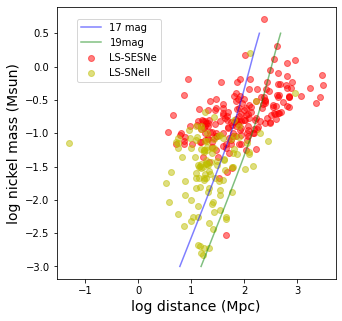
\includegraphics[width=\columnwidth]{Ni_vs_distance.png}
    \caption{The $^{56}$Ni masses of our samples as a function of the distance. The red points refer to LS-SESNe, while yellow points refer to LS-SNeII. For reference, the limiting distance for a given $^{56}$Ni mass estimated in section \ref{sec:relation} is also shown for the case of limiting magnitude of $V_{\mathrm{lim}} = 17$ (blue) and 19 mag (green).}
     \label{Ni_mass_vs_distance}
\end{figure}
In order to clarify how the observational biases may affect the $^{56}$Ni mass distribution in our samples, we look at the $^{56}$Ni mass of our samples as a function of the distance.
Figure \ref{Ni_mass_vs_distance} shows the $^{56}$Ni masses of our samples plotted as a function of the distance. It can be seen that there is a strong trend that the $^{56}$Ni mass decreases as the distance decreases for SESNe. This suggests that the objects with low $^{56}$Ni masses (i.e. dim objects) and large distance, if they exist, may be missed. It is, however, important to emphasize that we are still lacking the SESNe with low $^{56}$Ni mass (log $M_{\mathrm{Ni}} (M_{\odot}) \lesssim -1.7$: i.e., $M_{\mathrm{Ni}} \lesssim 0.02 M_{\odot}$) even at small distance (log distance (Mpc) $\lesssim 1$). For SNe II, even though the $^{56}$Ni mass slightly decreases as the distance decreases, the effect is much less significant than SESNe.


\begin{figure*}[htbp]
 \begin{center}
    \begin{tabular}{c}
    \begin{minipage}{0.5\hsize}
    \begin{center}
      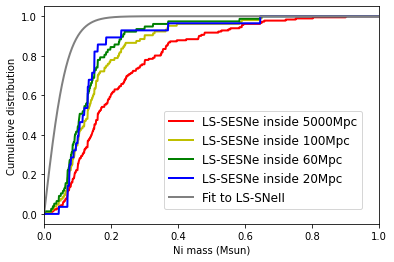
\includegraphics[width=85mm]{Ni_dist_different_d_cut_SESNe.png}
    \end{center}
  \end{minipage}
  \begin{minipage}{0.5\hsize}
    \begin{center}
       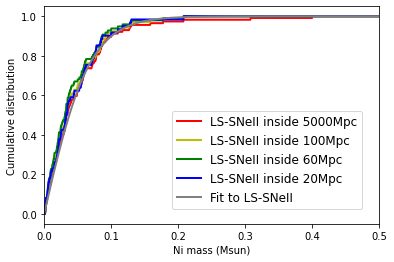
\includegraphics[width=85mm]{Ni_dist_different_d_cut_SNeII.png}
    \end{center}
  \end{minipage}
  \end{tabular}
 \end{center}
% \vspace{5zw}
 \caption{
 Left: The $^{56}$Ni mass distribution of LS-SESNe for the different sizes of volume-limited samples. The red cumulative distribution shows the $^{56}$Ni mass distribution of the samples among LS-SESNe whose distances are less than 5000 Mpc, while yellow, green and blue cumulative distributions show those whose distances are less than 100 Mpc, 60 Mpc and 20 Mpc, respectively. Right: The same figure as on the left plotted for LS-SNeII. For both figures, the non-linear least square fit to the LS-SNe II cumulative distribution is also shown with a gray line (See sec \ref{sec:ni_dist} for more detail).
 }
 %Left: The comparison of the normalized luminosity function of SESNe and SNe II sample. Right: The comparison of the normalized distance distribution of SESNe and SNe II sample.}
  \label{Ni_dist_different_d_cut}
\end{figure*}

\begin{figure}[htbp]
	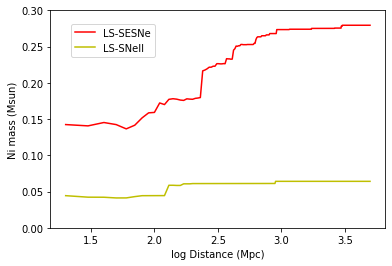
\includegraphics[width=\columnwidth]{Ni_volume_limited.png}
    \caption{The average $^{56}$Ni mass in the volume-limited sample plotted as a function of the threshold distance from 20 Mpc to 5000 Mpc. The red line refers to LS-SESNe sample, while yellow line refers to LS-SNeII.}
     \label{Ni_volume_limited}
\end{figure}

These trends can be confirmed by looking at Fig \ref{Ni_dist_different_d_cut} and \ref{Ni_volume_limited}. Figure \ref{Ni_dist_different_d_cut} shows how the $^{56}$Ni mass distribution changes when we take different sizes of volume-limited samples. It is expected that the $^{56}$Ni mass distribution approaches to the intrinsic distribution as we take the volume-limited sample at a closer location. It is seen that the $^{56}$Ni mass distribution of SESNe significantly shifts to the lower mass when we take the smaller volume-limited sample\footnote{Note, however, that the distributions for the lowest 20\% of the $^{56}$Ni masses are nearly the same for these different sizes of volume-limited samples. This may indicate that 
%only SESNe with relatively heavier $^{56}$Ni mass ($\gtrsim 0.1M_{\odot}$) suffer from the observational bias, and 
the lack of canonical SESNe with relatively low $^{56}$Ni mass ($\lesssim 0.02M_{\odot}$) is real. We will further discuss it in section \ref{sec:discussion}.}.
On the contrary, SNe II do not change notably for the different sizes of volume-limited sample. From this, we can infer that the LS-SESNe may not trace the intrinsic $^{56}$Ni mass distribution, while LS-SNeII nearly do. 

Figure \ref{Ni_volume_limited} shows the average $^{56}$Ni mass in the volume-limited samples plotted as a function of the threshold distance.  This figure, again, shows that LS-SESNe suffer from a significant observational bias and the discrepancy between SESNe and SNe II becomes smaller as we take the smaller volume-limited sample, and finally becomes within a factor of three.
%\textcolor{green}{Recently, \citet{2020arXiv200906683A} claimed that the $^{56}$Ni mass estimated using the `Arnett-rule' overestimates the value by a factor of two. Considering that the $^{56}$Ni masses for the majority of SESNe are estimated using the `Arnett-rule', the problem posed by }

%%% it means that the discrepancy between the $^{56}$Ni masses between SESNe and SNe II may nearly disappear, if we take a close volume-limited sample.
%実際どのくらい?

\begin{figure}[htbp]
	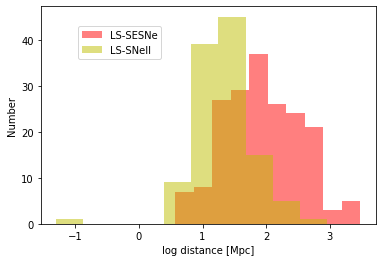
\includegraphics[width=\columnwidth]{D_dist_all.png}
    \caption{The comparison of the distance distributions of LS-SESNe (red) and LS-SNeII (yellow).}
     \label{D_dist_all}
\end{figure}

Figure \ref{D_dist_all} compares the distance distribution between LS-SESNe and LS-SNeII. We can see that the distance distribution is closer for SNe II than SESNe. 
\citet{2020A&A...641A.177M} showed that their 35 SESNe sample, excluding two Ic-GRB objects, have the mean distance (46.7 Mpc) similar to that of their SNe II sample (42.7 Mpc). However, our significantly larger sample of LS-SESNe has the mean distance of 226.6 Mpc, while LS-SNeII has the mean distance of 41.5 Mpc. Even if we remove Ic-BL and Ic-GRB from the SESNe sample, the mean distance is 99.8 Mpc, which is more than twice the value of LS-SNeII. This indicates that the SESNe samples are collected at more distant locations than SNe II, where the objects suffer from more significant observational bias, supporting the results derived above. 
\footnote{Although the samples in \citet{2020A&A...641A.177M} were taken at small distances ($\approx 40-50$ Mpc), the SESNe with low $^{56}$Ni mass ($\lesssim 0.02 M_{\odot}$) were still lacking.  Thus, the lack of canonical SESNe with relatively low $^{56}$Ni mass ($\lesssim 0.1M_{\odot}$) may actually be real. We will further discuss this point in section \ref{sec:discussion}.}

%The reason for this diffrence is 
%%Explain why.
\subsection{Luminosity distribution} \label{sec:l_func}

%\begin{figure}[htbp]
%	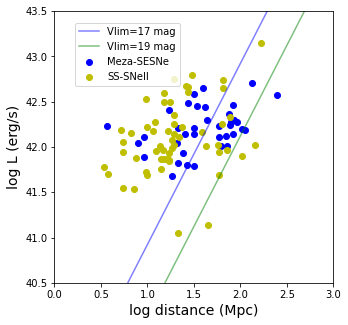
\includegraphics[width=\columnwidth]{Lpeak_dist.png}
%    \caption{The distributions of the peak luminosity of SESNe (red points) and plateau luminosity of SNe II (yellow points) plotted as a function of distance. For reference, the limiting luminosity as a function of distance is plotted for the case of limiting magnitude of $V_{\mathrm{lim}} = 17$ (blue line) and 19 mag (green line), respectively.}
%     \label{L_dist}
%\end{figure}

%\begin{figure}[htbp]
%	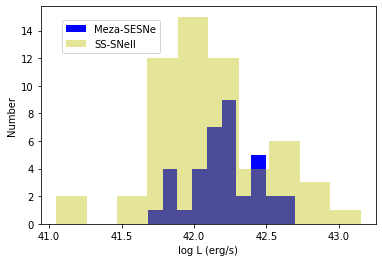
\includegraphics[width=\columnwidth]{Lfunc_compare.png}
%    \caption{The comparison of the luminosity function of SESNe (blue) and SNe II (yellow) sample. For SESNe, we show the peak luminosity, and for SNeII, we show the plateau luminosity.}
%     \label{Lfunc_compare}
%\end{figure}

\begin{figure*}[htbp]
    \begin{minipage}{0.5\hsize}
    \begin{center}
      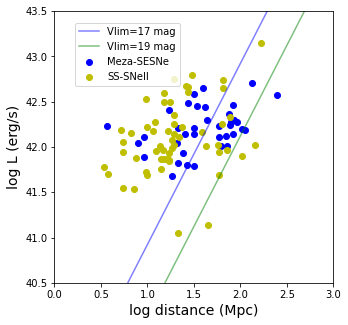
\includegraphics[width=85mm]{Lpeak_dist.png}
    \end{center}
  \end{minipage}
  \begin{minipage}{0.5\hsize}
    \begin{center}
       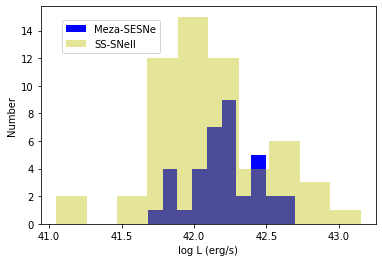
\includegraphics[width=85mm]{Lfunc_compare.png}
    \end{center}
  \end{minipage}
 \caption{Left: The distributions of the peak luminosity of SESNe (blue points) and plateau luminosity of SNe II (yellow points) plotted as a function of distance. For reference, the limiting luminosity as a function of distance is plotted for the case of limiting magnitude of $V_{\mathrm{lim}} = 17$ (blue line) and 19 mag (green line), respectively. Right: The comparison of the luminosity function of SESNe (blue) and SNe II (yellow) sample. For SESNe, we show the peak luminosity, and for SNeII, we show the plateau luminosity.}
 \label{L_funcs}
\end{figure*}

In this section, we investigate the luminosity distribution of our samples. We emphasise that the analysis in this section is not affected by the assumption about the relation between the $^{56}$Ni masses and the peak luminosity of SESNe.
As noted in section \ref{sec:sample}, here, we only use the sample of 57 SNeII taken from \citet{2003ApJ...582..905H, 2017ApJ...841..127M, 2015ApJ...806..225P}, which we call SS-SNeII. Note that \citet{2003ApJ...582..905H} only publishes the V-band magnitude, so, we convert it to bolometric luminosity assuming the bolometric correction to be zero, following \citet{2019ApJ...879....3G}. For SESNe, we use the sample of 37 from Meza-SESNe.

The left panel of Fig. \ref{L_funcs} shows the luminosity distribution as a function of distance for these samples. For SESNe we show the peak luminosity, while we show the plateau luminosity for SNe II. There is a positive correlation between the luminosity and distance both for SESNe and SNe II. Also, the minimum luminosity for a fixed distance is similar between SNe II and SESNe. This indicates that both of our samples may be suffering from the same observational selection effect.
The right panel of Fig. \ref{L_funcs} compares the luminosity functions of SESNe and SNe II. We notice that there is a luminosity cut off for both types at around log $L$[erg s$^{-1}$] $\sim 41.7$. The SNe II plateau phase and the SESNe peak phase are powered by the different physical mechanisms, with the former powered by the explosion energy and the latter powered by the radioactive decay of $^{56}$Ni. It is true the plateau luminosity and the $^{56}$Ni mass of SNe II are known to be positively correlated \citep{2015ApJ...806..225P}, but it is unlikely that the lower luminosity cut off are the same between the two groups of SNe just in terms of physics. Thus, we speculate that this simultaneous cut off of the luminosity functions for both types of SNe is caused by an observational selection effect.
This selection effect will introduce a bias in the $^{56}$Ni mass distribution for SESNe, as the $^{56}$Ni mass is closely connected to their peak luminosities.

%The median distance of our SESNe sample, excluding SNe Ic-BL and SNe Ic-GRB, is 47.8 and that of our SNe II sample is 29.8. On the contrary, \citet{2020arXiv200201015M} have derived the median distance of 46.7 Mpc for their SESNe sample, excluding SNe Ic-GRB, and of 42.7 Mpc for their sample of SNe II. The slight difference of the median distance between our SESNe sample and the SESNe sample in \citet{2020arXiv200201015M} is due to the exclusion of SNe Ic-BL in our sample. The median distance of our SNeII sample is smaller than the sample of \citet{2020arXiv200201015M}. Note that the size of SNe II sample used in this section is about a half of the size of SNe II sample used in \citet{2020arXiv200201015M}.

%Distances for our SE-SN sample are listed in Table A.1. Excluding the SNe Ic-GRB, the mean distance of this sample is
%46.7 Mpc. The 115 SNe II from Anderson have a mean distance of 42.7 Mpc. Thus there is little difference between the distances of the two samples. Given that SE-SN maximum-light luminosities are directly tied

To summarize, the results derived in section \ref{sec:investigate_obs_bias_from_datasample} 
all point to the following interpretation: {\it The $^{56}$Ni mass of SESNe samples collected from the published literature suffer from notable observational bias, i.e. the distant objects with relatively low $^{56}$Ni mass are missed, meaning that the samples are biased towards the luminous objects. On the contrary, the $^{56}$Ni masses of SNe II samples suffer much less from such bias.} We, again, emphasise that the analyses in this section are not affected by the assumption about the relation between the $^{56}$Ni masses and the peak luminosity of SESNe\footnote{We note, however, that \citet{2020A&A...641A.177M} have shown that the statistical difference of $^{56}$Ni mass between SESNe and SNe II remains even if they take relatively close samples ($\approx 40-50$ Mpc). Thus, the observational bias alone may not be sufficient to explain all of the statistical difference in the $^{56}$Ni mass (section \ref{sec:discussion}).}.

\section{Method of Mock observations} \label{sec:mock_obs}

In the previous sections, we have found that the $^{56}$Ni mass distribution in our SNe II sample is not notably suffering from the observational bias. Therefore, below, we start additional analysis based on the following two working hypotheses: (1) The $^{56}$Ni mass distribution in our SNe II sample (LS-SNeII) represents the intrinsic $^{56}$Ni mass distribution of SNe II, and (2) SESNe have the same intrinsic $^{56}$Ni mass distribution as that of SNe II. The second assumption is based on the hypothesis that
assuming a binary origin for SESNe, progenitors of SESNe and SNe II are expected to share the similar range in the initial mass (see section \ref{sec:intro})\footnote{Note, however, that there are indications that the progenitors of SESNe may be more massive than SNe II either as an entire class or for the particular SN Ic class \citep[e.g.][]{2012MNRAS.424.1372A, 2012ApJ...749L..28V, 2019NatAs...3..434F}.}.

Based on these hypotheses, we conduct mock observations of SESNe.
%, i.e; we trigger a fixed number of SESNe with the random values of $^{56}$Ni mass taken from the same probability distribution as SNe II and
By comparing the results of mock observations to the data sample, we discuss the reliability of these hypotheses. In the rest of this section, we describe the procedure of the mock observation in more detail.

\subsection{$^{56}$Ni mass distribution} \label{sec:ni_dist}
As noted above, here we assume that the intrinsic $^{56}$Ni mass distribution of SESNe is the same as the $^{56}$Ni mass distribution of LS-SNe II.
%%% Citation!!! %%%%
%For the $^{56}$Ni mass distribution of SNe II, we use the LS-SNeII sample. 
To simplify the numerical analyses, we fit the cumulative histogram of $^{56}$Ni mass (denoted here as $f(x)$) by the function of $f(x) =$tanh$(a_0 \times x)$, using non-linear least squares. We obtained $a_0= 14.60$ as the best fit parameter. The comparison of our fitted curve with our sample is shown in Fig. \ref{fit_data}. Below, we use the function of $f(x)$= tanh$(14.60 \times x)$ to represent the $^{56}$Ni mass distribution of SESNe. 

\begin{figure}
	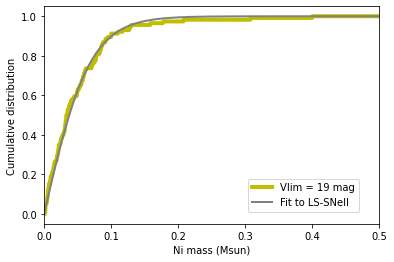
\includegraphics[width=\columnwidth]{Ni_fit.png}
    \caption{The cumulative $^{56}$Ni mass distribution of LS-SNeII
    and the non-linear least squares fit to it, assuming the function of $f(x)= $tanh$(a_0 \times x)$.}
     \label{fit_data}
\end{figure}

\subsection{Simulating the observations}
We simulate one SESN by selecting the $^{56}$Ni mass and distance from the given probability distributions. We select a value of $^{56}$Ni mass from the distribution derived in section \ref{sec:ni_dist}. Then, for each $^{56}$Ni mass thus derived, the distance is randomly chosen following the probability function of $p \propto$ (distance)$^3$, i.e., the volume size. The range of distance is set from zero up to the limiting distance corresponding to the peak luminosity of SESNe with a $^{56}$Ni mass of 1.0$M_{\odot}$.

For each object with a given $^{56}$Ni mass and distance, we decide whether to add it to the `detected' sample or not based on the following procedure. First, from the given $^{56}$Ni mass, we estimate the peak luminosity as described in \ref{sec:relation}. Next, we can estimate the limiting distance using equation \ref{d_lim_eq}, for the peak luminosity derived above. 
If the selected distance is within the observable distance corresponding to its peak luminosity, we consider it to be detected and add it to the detected sample. Otherwise, we consider that the object escapes detection and do not add it to the detected sample. Once the number of detections reaches 100, we stop one iteration of the mock observation. The number of 100 is chosen to be consistent with the order of magnitude of our LS-SESNe sample size. Note, however, that only in section \ref{sec:lfun_mock}, we set this number as 37 (i.e., the Meza-SESNe sample size) in order to make a direct comparison to Meza-SESNe. We iterate the procedure described above $10^3$ times, in order to clarify the possible range of the distributions by taking into account the statistical fluctuation due to the limited sample size.

\section{Results of mock observation} \label{sec:mock_result}

\subsection{Luminosity function} \label{sec:lfun_mock}
\begin{figure}[htbp]
	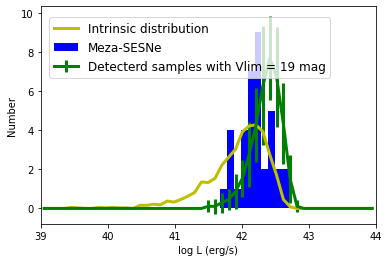
\includegraphics[width=\columnwidth]{L_dist_compare_intrinsic_to_observed.png}
    \caption{The luminosity functions derived from the mock observation are compared to the luminosity function of Meza-SESNe (blue). The yellow histogram is the distribution of the detected samples in the mock observation assuming that all objects are detected regardless of their distances, i.e; this traces the intrinsic luminosity function of SESNe (assuming that this is the same as that of SNeII). The green histogram is the luminosity function of the detected sample in the mock observation, assuming the limiting magnitude of 19 mag. For the green line, the solid line represents the mean distribution of 1000 iterations of 37 detections and the error bar is the standard deviation of 1000 distributions in each bin.}  
     \label{L_dist_mock_compare_19_to_data}
\end{figure}

Here, we show the results of the mock observation described in section \ref{sec:mock_obs}. We assume a fixed limiting magnitude of 19 mag in this section. Figure \ref{L_dist_mock_compare_19_to_data} compares the luminosity functions derived from the mock observations to the luminosity function of Meza-SESNe\footnote{The reason for the non-smooth intrinsic distribution in Fig. \ref{L_dist_mock_compare_19_to_data} is the small number (i.e., 37) of detections we assumed.}. Here, in order to make the direct comparison to Meza-SESNe, we stop one iteration of mock observation when the number of detected objects reaches 37 (i.e., the Meza-SESNe sample size), not 100. Then, we repeat this 1000 times to clarify the possible range of the distributions.

Interestingly, we can see that the luminosity function in the `detected' samples is shifted to high luminosity compared to the model intrinsic luminosity function. Since the objects with higher luminosity (i.e., higher $^{56}$Ni mass) have the larger observable volume, they dominates the detected sample.
It is also worthwhile to note that the luminosity function of our detected samples in the mock observation roughly explains the observed luminosity function of Meza-SESNe. Especially, the lower cut-off at around log $L \sim 41.7$ is naturally obtained. 

%The reason for the non-smooth intrinsic distribution is the small number (i.e., 37) of detections we assumed.

\subsection{$^{56}$Ni mass distribution} \label{sec:Nimass_moock}
\begin{figure}[htbp]
	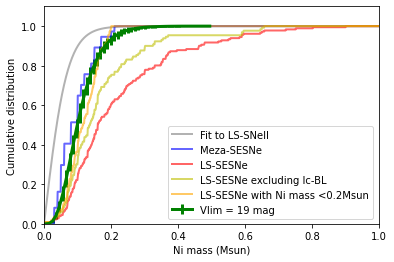
\includegraphics[width=\columnwidth]{Ni_dist_compare_19_to_data.png}
    \caption{The $^{56}$Ni mass distribution in the detected sample of our mock observation (green) is compared to Meza-SESNe (blue) and LS-SESNe (red). The $^{56}$Ni mass in Meza-SESNe is the value estimated using the `Arnett-rule'. The green solid line represents the mean distribution of 1000 iterations of 100 detections and the error bar is the standard deviation of 1000 iterations in each bin. For reference, a sub-sample derived from LS-SESNe by removing Ic-BL is colored with yellow, while a sub-sample of LS-SESNe which satisfies $M_{\mathrm{Ni}} \leq  0.2M_{\odot}$ is colored with orange. Also, the fit to the $^{56}$Ni mass distribution  of LS-SNe II is shown with a gray line.} 
     \label{Ni_dist_mock_compare_19_to_data}
\end{figure}

Figure \ref{Ni_dist_mock_compare_19_to_data} compares the cumulative $^{56}$Ni mass distribution in the detected samples to different data samples. Note that, below, we stop one iteration of mock observation when the number of detect objects reaches 100.
The $^{56}$Ni mass distribution in the detected sample of our mock observation is skewed to higher mass compared to the assumed intrinsic distribution. This is due to the observational bias, being consistent with the shift of the luminosity function discussed in the previous section. %Interestingly, the predicted $^{56}$Ni mass distribution lies in the intermediate between Meza-SESNe and LS-SESNe.
The predicted $^{56}$Ni mass distribution is very close to that of Meza-SESNe, which consists of well-observed objects.
From this, we again emphasize that the systematically high $^{56}$Ni masses in the SESNe sample compared to those of SNe II sample could, at least partly, be explained by the observational bias.

The larger sample LS-SESNe, however, contains more massive objects than Meza-SESNe, which are not explained by our mock observations.
If we remove the objects with $M_{\mathrm{Ni}} \gtrsim 0.2M_{\odot}$ from LS-SESNe, it matches with the prediction of mock observations much better. This might indicate that the objects with  $M_{\mathrm{Ni}} \gtrsim 0.2M_{\odot}$ are triggered by a different explosion mechanism from the objects with lower $^{56}$Ni masses (see section \ref{sec:discussion}). 

%%% KS-test???

%Fig. \ref{Distance_dist_mock_to_data} compares the histogram of distance of our SESNe sample to the results of the mock observations for the different limiting magnitudes. Although the results of our mock observation does not explain the distance distribution of our sample, it is natural considering that our sample consists of various surveys with the various limiting magnitude. 

\subsection{Effect of different limiting magnitudes} \label{sec:different_vlim}

\begin{figure}[htbp]
	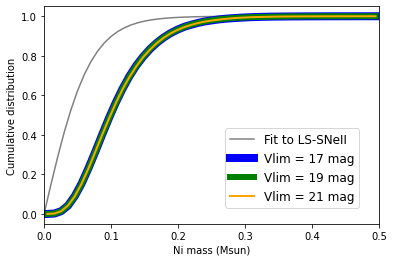
\includegraphics[width=\columnwidth]{Ni_cum_dist_different_Vlim.png}
    \caption{The cumulative $^{56}$Ni mass distribution of the detected samples in the mock observation for the different limiting magnitudes. Blue, green, orange lines refer to the limiting magnitude of 17 mag, 19 mag, and 21 mag, respectively. Each line is the mean of the distributions derived from 1000 iterations. For reference, the fit to the $^{56}$Ni mass distribution  of LS-SNe II is shown with a gray line.} 
     \label{Ni_dist_mock_different_Vlim}
\end{figure}

In the previous section, we have assumed a limiting magnitude of Vlim = 19 mag. Next, we will see how the different values of the limiting magnitudes affect our results.
In Fig. \ref{Ni_dist_mock_different_Vlim}, we show the $^{56}$Ni mass distribution of the detected samples in the mock observation for the different limiting magnitudes. We can see that the $^{56}$Ni mass distribution is quite insensitive to the different values of the limiting magnitudes. This can be explained as follows. The $^{56}$Ni mass distribution in the observed sample can be derived by multiplying the assumed intrinsic distribution of $^{56}$Ni mass by $D_{\mathrm{lim}} (M_{\mathrm{Ni}})^3$. Here,
$D_{\mathrm{lim}} (M_{\mathrm{Ni}})$  is the limiting distance calculated using equation \ref{d_lim_eq}. Thus, the term of $V_{\mathrm{lim}}$ only changes the scale of the $^{56}$Ni mass distribution, but does not affect the normalized distribution. 
Thus, we can say that the results derived in the previous section is robust to the different limiting magnitudes that are assumed. 
%%%% Explain why %%%%%%

\begin{figure}[t] %[htbp]
	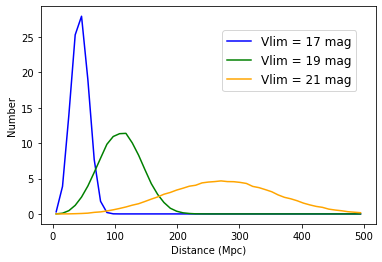
\includegraphics[width=\columnwidth]{Distance_distribution_different_Vlim.png}
    \caption{The distance distribution of the detected samples in the mock observation for the different limiting magnitudes. Blue, green, orange lines refer to the limiting magnitude of 17 mag, 19 mag, and 21 mag, respectively. Each line is the mean of the distributions derived from 1000 iterations.} 
     \label{Distance_dist_mock_different_Vlim}
\end{figure}

In Fig. \ref{Distance_dist_mock_different_Vlim}, we show the distance distribution of the detected samples in the mock observation for the different limiting magnitudes. We can see that the distance distribution is sensitive to the different value of the limiting magnitude. The higher the limiting magnitude is, the observable volume becomes larger. Thus, the more distant objects dominates the observed sample.

\begin{figure*}[htbp]
 \begin{center}
    \begin{tabular}{c}
    \begin{minipage}{0.5\hsize}
    \begin{center}
      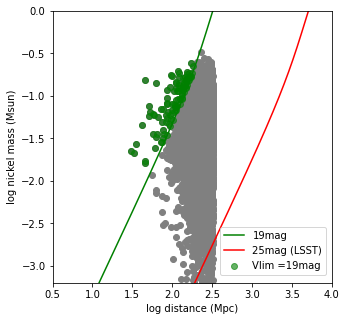
\includegraphics[width=85mm]{Ni_vs_distance_wt_mock_no_obs_data.png}
    \end{center}
  \end{minipage}
  \begin{minipage}{0.5\hsize}
    \begin{center}
       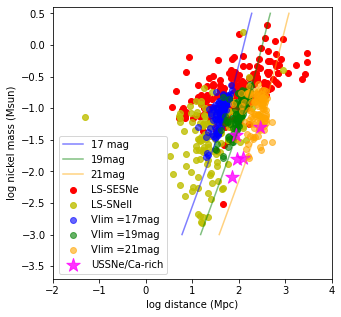
\includegraphics[width=85mm]{Ni_vs_distance_wt_mock.png}
    \end{center}
  \end{minipage}
  \end{tabular}
 \end{center}
 \caption{Left: The $^{56}$Ni mass and distance of the detected samples in one iteration (i.e., 100 detections) for the limiting magnitudes of 19 mag. Gray points are all the events that were randomly picked up until the number of detections reached 100. For reference, the limiting distance for a given $^{56}$Ni mass estimated as in section \ref{sec:relation} are also shown assuming the limiting magnitudes of 19 (green) and 25 (red) mag. The latter represents the limiting magnitude for the single-visit depth in LSST \citep{2019ApJ...873..111I}.
 Right: The $^{56}$Ni mass and distance of the detected samples in one iteration for the different limiting magnitudes. Blue, green, orange points refer to the case of limiting magnitude of 17 mag, 19 mag, and 21 mag, respectively. We add the ultra-stripped envelope SNe (USSNe) candidates with magenta star marks (see section \ref{sec:discussion} for a discussion of these events). The references for USSNe are listed at the end of the manuscript. For both panels, the limiting distance for a given $^{56}$Ni mass estimated as in section \ref{sec:relation} are also shown assuming the fixed limiting magnitudes. }
  \label{Ni_vs_dist_dist_mock_different_Vlim}
\end{figure*}




In the right panel of Fig. \ref{Ni_vs_dist_dist_mock_different_Vlim}, the $^{56}$Ni masses and distances of the detected samples for the different limiting magnitudes are over-plotted onto Fig.\ref{Ni_mass_vs_distance}. As discussed above, the objects with low $^{56}$Ni mass are lacking compared to the assumed intrinsic distribution, which is consistent with the data samples. However, it is important to note that our predictions from the mock observations fail to explain the high $^{56}$Ni masses of $\gtrsim 0.2 M_{\odot}$ that exist in the data samples collected from the published literature as already noted in section \ref{sec:Nimass_moock}. 

\subsection{Effects of different observational cadences}
So far, we implicitly assumed an infinitely small observational cadence in the mock observation. This means that an object is always detected as long as its peak luminosity exceeds the observational limiting magnitudes. However, existing surveys have a wide range of observational cadence from hours to a few tens of days, depending on their scientific aims. Therefore, some objects may be missed due to to infrequent observations, even if the peak luminosity exceeds the observational limiting magnitudes. 
Therefore, here we attempt to take this into account. Following this, we investigate how the different observational cadences affects our results. We fix the limiting magnitude as 19.0 mag in this section for simplicity.

To proceed with this investigation, we take a simplified approach. We assume that the peak luminosity is maintained for the duration of $t_p$ calculated using equation \ref{eq:t_p}. For the ejecta mass and explosion energy that appear in equation \ref{eq:Lpeak} and \ref{eq:t_p}, we use the relations in equation \ref{Mej_MNi} just as we have done in the analyses so far. We simulate the values of observational cadence of 0.0, 10.0, 20.0, 30.0 days.
In the mock observation, we add a procedure as follows, 
in order to decide whether an object is detected or not: if the duration of the event is less than the observational cadence, we add it to the observed sample with the probability of $p = t_p/t_\mathrm{cadence}$. If the duration of the event is longer than the observational cadence, we consider the object is detected and add it to the observed sample.

\begin{figure}[t]
	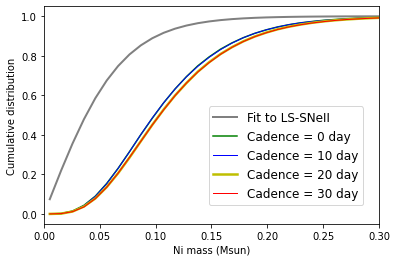
\includegraphics[width=\columnwidth]{Ni_cum_dist_different_cadence.png}
    \caption{The $^{56}$Ni mass distribution of the detected samples for the different observational cadences. 
    Green, blue, yellow, and red points refer to the cadence of 0.0, 10.0, 20.0, 30.0 days, respectively. Each line is the mean of the distributions derived from 1000 iterations. 
    For reference, the fit to the $^{56}$Ni mass distribution  of LS-SNe II is shown with a gray line.} 
     \label{Ni_dist_different_cadence}
\end{figure}

\begin{figure}[htbp]
	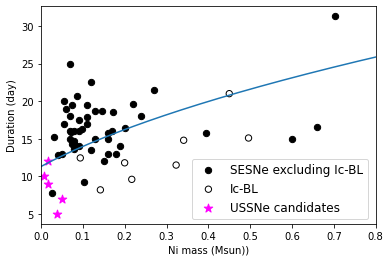
\includegraphics[width=\columnwidth]{Ni_vs_tau.png}
    \caption{The estimated duration of SESNe using equation \ref{eq:t_p} plotted as a function of $^{56}$Ni mass. For reference, the observational data taken from \citet{2016MNRAS.457..328L} and \citet{2019MNRAS.485.1559P} are also shown with black points. Among them, open circles are the SNe Ic-BL, while the filled circles are the other types of SESNe. Also, the data of USSNe candidates are also shown with magenta star marks, which are taken from the reference list attached at the end of the manuscript.} 
     \label{Ni_vs_tau}
\end{figure}

Figure \ref{Ni_dist_different_cadence} compares the $^{56}$Ni mass distribution of the detected samples for the different observational cadences. It is seen that the difference is negligible.
This is because the timescale of SESNe within our formalism is not particularly sensitive to the $^{56}$Ni mass as shown in Fig. \ref{Ni_vs_tau}. Thus, we conclude that our results are robust to the different assumptions about the observational cadences. 
However, note that Fig. \ref{Ni_vs_tau} is based on the linear fitting equations \ref{eq:Mej_Ek_MNi}. This fitting is done using the samples with $^{56}$Ni masses above $0.03M_{\odot}$, and the validity of the linear extrapolation to the lower $^{56}$Ni masses is not trivial (see, section \ref{sec:discussion}).

\section{Discussion} \label{sec:discussion}
In section \ref{sec:investigate_obs_bias_from_datasample}, we found that the $^{56}$Ni masses of SESNe samples collected from the published literature suffer from notable observational bias, while those of SNe II samples suffer from much less bias. This may be because: (1) SNe II samples are collected at closer distances compared to SESNe samples (Fig. \ref{D_dist_all}), meaning that the former suffer less bias; or (2) the luminosity of SESNe have higher dependence on the $^{56}$Ni mass than SNe II. Indeed, the peak luminosity of SESNe is theoretically expected to follow $L_{\mathrm{peak}}\propto M_{\mathrm{Ni}}$ \citep{1982ApJ...253..785A}, while the mid-plateau luminosity of SNe II is phenomenologically known to follow $L_{\mathrm{plateau}} \propto M_{\mathrm{Ni}}^{0.65}$ \citep{2015ApJ...806..225P}. Moreover, at the early phase, SNe II generally have higher luminosity than the mid-plateau phase. Thus, the detectability of SNe II is affected much less by $^{56}$Ni mass than SESNe.  

We have conducted mock observations and shown that if we assume that the intrinsic $^{56}$Ni mass distribution of SESNe is the same as that of LS-SNe II, the $^{56}$Ni mass distribution of SESNe in the detected samples becomes more massive compared to the assumed intrinsic distribution, which is very close to the distribution of Meza-SESNe. 
%suggests that our working hypothesis may explain the statistical differences between SESN and SN~II $^{56}$Nimasses previously found. 
This indicates that even if a significant number of SESNe with low $^{56}$Ni masses (i.e. similar to those low $^{56}$Ni SNe II masses) exists, we would find difficulty in detecting them and thus they would be significantly underrepresented in current literature samples.

However, some problems still remain to be solved. It is true that our mock observations predict that the detection of SESNe is dominated by relatively luminous objects. But, there should be at least a few SESNe with low $^{56}$Ni mass, $M_{\mathrm{Ni}} \lesssim 0.02 M_{\odot}$,  especially at small distances, considering that many SNe II with such low $^{56}$Ni masses are detected. However, in our samples, very few SESNe have been found with such low $^{56}$Ni mass. Of course, it may indicate that SESNe with such low $^{56}$Ni masses actually do not exist and the statistical difference of $^{56}$Ni mass between SESNe and SNe II is real. But, it may also be possible that the SESNe with low $^{56}$Ni mass  do not appear as canonical SESNe and instead appear as peculiar objects which are difficult to detect.


First, such low-$^{56}$Ni mass SESNe may be related to the so called rapidly evolving transients. As shown in Fig. \ref{Ni_vs_tau}, the $^{56}$Ni mass and the timescale of SESNe are known to be positively correlated: i.e., SESNe with lower $^{56}$Ni mass are expected to have shorter timescales. If we remove the SNe Ic-BL, which are considered to be quite different from the other types of SESNe, the timescale of SESNe decreases more rapidly than our prediction (Fig. \ref{Ni_vs_tau}).
%Also, ultra-stripped envelope SNe (USSNe) candidates have much shorter timescales than our prediction. 
Thus, our linear fit (section \ref{sec:relation_SESNe}) may not be valid at small $^{56}$Ni masses, and it can be possible that SESNe with low $^{56}$Ni mass ($\lesssim 0.02M_{\odot}$) are observed as rapidly evolving transients with timescales shorter than 10 days\footnote{Note, that some of the rapidly evolving transient are known to be difficult to explain by only considering the radioactive decay model \citep[e.g.][]{2014ApJ...794...23D}. However, the properties of the rapidly evolving the transients are diverse \citep{ 2018MNRAS.481..894P} and there are many that are compatible with the radioactive decay scenario.}
Actually, SN 2017czd in our sample is a SN IIb with very small $^{56}$Ni mass of $0.003M_{\odot}$. This object is classified also 
as a rapidly evolving transient \citep{2019ApJ...875...76N}. \citet{2014ApJ...794...23D} have estimated that the rate of rapidly evolving transients is 4-7 \% of the core collapse SNe rate. Since the fraction of SESNe in the core collapse SNe is 36.6 \% \citep{2011MNRAS.412.1522S}, the rapidly evolving transients occupy 11-19 \% of SESNe. This number is comparable to the fraction of SESNe with $M_{\mathrm{Ni}} \lesssim 0.01 M_{\odot}$ assuming the same $^{56}$Ni mass distribution as LS-SNeII. Since the events with short timescales ($\lesssim 10$ days) can be easily missed, this hypothesis may be consistent with the lack of SESNe with low $^{56}$Ni masses ($\lesssim 0.02 M_{\odot}$)\footnote{Note, that most of the rapidly evolving transient discovered so far have $^{56}$Ni mass of $\gtrsim 0.03 M_{\odot}$ \citep{2014ApJ...794...23D, 2018MNRAS.481..894P, 2020ApJ...894...27T}. However, considering that the number of samples detected so far is limited ($\approx 100$) \citep{2018MNRAS.481..894P}, it is natural that they are dominated by the relatively luminous objects as we have shown in section \ref{sec:mock_result}.}


%If the SESNe with low $^{56}$Ni mass appear as rapidly evolving transients instead of canonical SESNe, we may explain why the SESNe with low $^{56}$Ni of $\lesssim 0.02 M_{\odot}$ are lacking in LS-SESNe. That is, their short timescales ($\lesssim$ 10 days) make it difficult to detect them. Thus, the rapidly evolving transients are the possible counterparts for the SESNe with low $^{56}$Ni mass ($\lesssim 0.02 M_{\odot}$).
%Note, however, that some of the rapidly evolving transient are known to be difficult to explain by only considering the radioactive decay model. Also, many of the rapidly evolving transients known so far have $^{56}$Ni mass of $\gtrsim 0.03 M_{\odot}$ \citep{2014ApJ...794...23D, 2020ApJ...894...27T}. Thus, they may not be sufficient to explain all of the deficit of the SESNe with low $^{56}$Ni mass.

The SESNe with low $^{56}$Ni mass may also originate from the so-called ultra-stripped envelope SNe (USSNe). Actually, the ejecta mass and $^{56}$Ni mass of SESNe are known to be positively correlated \citep{2016MNRAS.457..328L}. Thus, the ejcta mass of the SESNe with low $^{56}$Ni mass are expected to be small. In Fig. \ref{Ni_vs_dist_dist_mock_different_Vlim}, the USSNe candidates are also shown. They have the $^{56}$Ni mass lower than most of our SESNe sample. Theoretical calculations also indicate that USSNe should synthesize quite low $^{56}$Ni of $\sim 0.01 M_{\odot}$ \citep{2015MNRAS.454.3073S, 2017MNRAS.466.2085M}. 
Specifically, SN2019dge, an USSNe candidate, has an estimated $^{56}$Ni mass of 0.017$M_{\odot}$ \citep{2020ApJ...900...46Y}, which is quite low. The rate of such events is estimated as 2-12\% of core collapse supernova: i.e., 5.6-33.3\% of SESNe \citep{2011MNRAS.412.1522S}.
%Considering that SESNe occupy 36.6\% of core collapse SNe \citep{2011MNRAS.412.1522S}, this means that such objects occupy 5.6-33.3\% of SESNe.
This number is consistent with the fraction of SESNe with $M_{\mathrm{Ni}} \lesssim 0.02 M_{\odot}$ under the distribution we assumed.
 Furthermore, the timescale of USSNe candidates are known to be short ($\lesssim 10$ days), which is much less than our prediction (Fig. \ref{Ni_vs_tau}).
 %Such short timescales may explain why we are missing them at small distances. 
Such short-timescale objects may be systematically non-detected in the existing surveys as noted in the previous paragraph.  
 % Thus, USSNe may be the possible candidate for the SESNe with low $^{56}$Ni mass ($\lesssim 0.02 M_{\odot}$). 
Note, however, that the $^{56}$Ni masses of USSNe candidates discovered so far are in general not too low: i.e., many SNe II have been detected with $^{56}$Ni mass lower than these objects. Therefore, these objects alone may not be sufficient to explain the deficit 
of SESNe with low $^{56}$Ni mass.

The SESNe with low $^{56}$Ni mass may also have the possible link to SNe Ibn, which are not included in our samples. SN Ibn is a explosion characterized by He emission line that is considered to originate from the interaction with the He-rich material. These objects are considered to eject less $^{56}$Ni than the bulk of other SESNe  \citep{2016ApJ...824..100M}.

% Ouchi_memo: ejecta mass とか Mejはlinear fitでは説明できなさそう。これは線形fitが成り立たないことを示唆しているかも。


%Although the $^{56}$Ni mass distribution from our mock observation may explain the general trend in the SESNe data sample, i.e; lack of low $^{56}$Ni mass objects, 
It is also important to note that our predictions from the mock observations fail to explain the high $^{56}$Ni masses of $\gtrsim 0.2 M_{\odot}$, which occupy a significant fraction of LS-SESNe (sections \ref{sec:Nimass_moock} and \ref{sec:different_vlim}).
% Thus, for the objects with high $^{56}$Ni ($\gtrsim 0.3 M_{\odot}$), other explanation might be needed. 
One possibility for this is that such objects with high $^{56}$Ni mass are triggered by a different explosion mechanism from the objects with lower $^{56}$Ni masses. Actually, as shown in Fig. \ref{Ni_dist_mock_compare_19_to_data}, the mock observation explains the data sample much better, if we remove the objects with $M_{\mathrm{Ni}} \gtrsim 0.2M_{\odot}$ from LS-SESNe. Note that SNe Ic-BL, whose $^{56}$Ni mass is significantly higher than the rest of SESNe \citep{2019A&A...628A...7A}, are considered to be triggered by a different explosion mechanism from the other types of SESNe \citep{2012ApJ...750...68L, 2018ApJ...860...38B}. Thus, the objects with $M_{\mathrm{Ni}} \gtrsim 0.2 M_{\odot}$ might be triggered by the similar mechanism as Ic-BL. The fraction of objects with $M_{\mathrm{Ni}} \gtrsim 0.2 M_{\odot}$ among LS-SESNe is 42 \%, while that of Ic-BL is 30 \%, which are not so different.

The difference in the $^{56}$Ni mass can also be caused by a different initial mass range of SESNe progenitors from that of SNe II. Current observational evidence favors the scenario that the mass stripping in SNe IIb/Ib progenitor is caused by binary mass transfer rather than the extensive stellar wind of a massive star ($M_{\mathrm{ms}} \gtrsim 25 M_{\odot}$) \citep{1994ApJ...429..300W, 2013ApJ...762...74B, 2015ApJ...811..147F}. However, there are several indications that at least a fraction of SESNe progenitors may be more massive than those of SNe II \citep[e.g.][]{2012MNRAS.424.1372A, 2018MNRAS.476.2629M, 2019NatAs...3..434F}. This may imply that our assumption that SESNe share the same $^{56}$Ni mass distribution as SNe II may be too simplified.

%The fraction of objects with $M_{\mathrm{Ni}} \gtrsim 0.3M_{\odot}$ among LS-SESNe is 24\%. This number is very close to the fraction (22\%) of Ic-BL among the samples in 
%\citet{2019A&A...628A...7A}. This might indicate that there might be roughly the same number of objects as Ic-BL that are triggered by the same mechanism as Ic-BL, that are not classified as Ic-BL.


Another possibility is that different amounts of fall back may occur between SNe~II and SESNe. SNe II have the thick hydrogen envelope outside the He core, and the shock is decelerated while crossing the envelope. Thus, it is expected that SNe II suffer from fall back of the inner material more substantially than SESNe. In this case, the $^{56}$Ni mass distribution of SNe II we have used may be a lower limit (Sawada et al. in prep). 



Throughout the paper, we have contrasted the SNe II to SESNe in general. \citet{2019A&A...628A...7A} has suggested that there may be difference of the $^{56}$Ni mass distribution even among the different types of SESNe. Especially, SNe IIb seem to have smaller $^{56}$Ni than SNe Ib/Ic. This might be explained in that SNe IIb can be detected more easily than SNe Ib/Ic due to their cooling emission. However, investigating this possibility quantitatively is beyond the scope of this paper.

%When deep surveys like LSST are deployed in the future, it will be worthwhile to construct a larger volume-limited samples and recreate the $^{56}$Ni mass distribution for SESNe. By doing so, we can further test our hypotheses. 
% (I should study more about LSST.)
When deep surveys like LSST are deployed in the future, we can test our hypotheses. In the left panel of Fig. \ref{Ni_vs_dist_dist_mock_different_Vlim}, we show the detection limit for a limiting magnitude of 25 mag, representing the single-visit depth in LSST \citep{2019ApJ...873..111I}. We can see that basically all the SESNe with low $^{56}$Ni masses  ($\lesssim 0.02 M_{\odot}$) are detected if they occur closer than $\approx 100$ Mpc\footnote{Although there are many objects with $M_{\mathrm{Ni}} \lesssim 10^{-3} M_{\odot}$ in the left panel of Fig.\ref{Ni_vs_dist_dist_mock_different_Vlim}, they are considered to be an artifact caused by an analytical fitting to the distribution, considering that there are no such objects in LS-SNe II (section \ref{fit_data}).} Thus, we will be able to construct a complete sample of SESNe in the local universe. With such a sample, we can test whether the lack of SESNe with $\lesssim 0.02 M_{\odot}$ is real or not.

%it will be worthwhile to construct a larger volume-limited samples and recreate the $^{56}$Ni mass distribution for SESNe. By doing so, we can further test our hypotheses. 


\section{Conclusion} \label{sec:conclusion}
The nuclear decay of $^{56}$Ni is one of the most important power sources of supernovae (SNe). Recent works have indicated that the $^{56}$Ni masses estimated for SESNe are systematically higher than those estimated for SNe II. Although this may indicate distinct progenitor structure or explosion mechanism between these types of SNe, the possibility remains that this may be caused by observational biases. 

By investigating the distributions of $^{56}$Ni mass and distance for the data samples collected from the literature, we have found that SESNe samples suffer from significant observational bias; objects with low $^{56}$Ni masses may be systematically missed, especially at larger distances. 
Thus, this work has elucidated that the observational bias must be taken into account in discussing the different $^{56}$Ni masses between SNe II and SESNe.

We also conducted mock observations assuming that the intrinsic $^{56}$Ni mass distribution of SESNe is the same as the $^{56}$Ni mass distribution of SNe II collected from the literature. We have found that the $^{56}$Ni distribution for the detected samples of SESNe becomes more massive compared to the assumed intrinsic distribution due to the observational bias. This result may, at least partially, explain the lack of low $^{56}$Ni mass objects in the SESNe data sample collected from the literature. Although this result relies on the assumption noted above, this supports that at least a part of the  systematically different $^{56}$Ni masses between these types of SNe are due to the observational bias. 

We emphasize, however, that the SESNe with low $^{56}$Ni mass ($\lesssim 0.02 M_{\odot}$) are still lacking even at small distances ($\lesssim$ 30 Mpc). This may indicate that the observational bias alone may not be sufficient to explain all of the statistical difference between SESNe and SNe II. Another possibility is that the SESNe with low $^{56}$Ni mass appear as either rapidly evolving transients or ultra-stripped SNe, which are difficult to detect due to their short timescales.

%\appendix
%\section{Derivation of luminosity distribution}
\section{acknowledgement}
R.O. acknowledges support provided by Japan Society for the Promotion of Science (JSPS) through KAKENHI grant (19J14158).
K.M. acknowledges support provided by Japan Society for the Promotion of Science (JSPS) through KAKENHI grant (18H05223, 20H00174, and 20H04737). This work is partly supported by the JSPS Open Partnership Bilateral Joint Research Project between Japan and Chile. 

%The probability function of $x(\equiv M_{\mathrm{Ni}})$ is \[f(x)= (\mathrm{tanh}(a0\times x))'= a_0/\mathrm{cos}^2\mathrm{h}(a_0\times x)\]. Therefore, the probability function of $y(\equiv M_{\mathrm{peak}}) = h(x)$ can be written as 
%\begin{eqnarray}
%    g(y) = f(h^{-1}(y)) |(h^{-1})'(y)|. 
%\end{eqnarray} 

%log10 MNi = −0.415 × Mpeak − 8.184.




\begin{comment}
F is the distribution function. i.e. F(x) means the the probability of X less than x is F(x). Note that $h(x)=-2.410 \mathrm{log}10(x) - 19.721$ and $F(x) = \mathrm{tanh}(a0\times x)$.



\begin{eqnarray}
F^{Y} (x) &=& P(Y<x) \\
&=& P(h^{-1}(x)<X) \\
&=& 1 - P(X< h^{-1}(x)) \\
&=& 1 -F(h^{-1}(x)).
\end{eqnarray}

The probability function for Y 


%%%%%%%%%%%%%%%%%%%%%%%%%%

\citet{2016MNRAS.457..328L} has compared the $^{56}$Ni mass and peak luminosity for SESNe, and derived the tight relation of 
\[\mathrm{log}_{10}  M_{\mathrm{Ni}} = -0.415 \times M_{\mathrm{peak}} -8.184.
\]
From this relation and the $^{56}$Ni mass distribution (Fig.\ref{fit_data}), we can derive the probabity function of the peak magnitude for the SESNe. The estimated distribution is shown in Fig.\ref{L_dist}. The detailed derivation for this relation is shown in appendix. Also shown in this figure are the distributions of peak magnitude derived in  \citet{2020A&A...641A.177M} and \citet{2016MNRAS.457..328L}. 



%\[
%M_{\mathrm{peak}} = -2.4096 \times \mathrm{log}_{10} %\mathrm{tanh}(a0 \times x)- 19.7205
%\]


\begin{figure}
	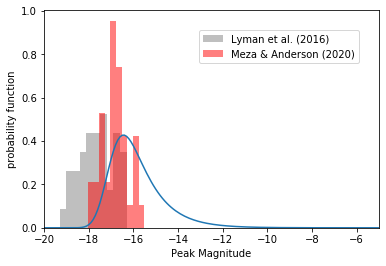
\includegraphics[width=\columnwidth]{L_dist.png}
    \caption{The estimated distribution of peak magnitude, assuming the same $^{56}$Ni distribution for SESNe as that of SNe II. The distribution of SESNe shown in \citet{2020A&A...641A.177M} and \citet{2016MNRAS.457..328L} are also shown with red and gray color, respectively.} 
     \label{L_dist}
\end{figure}



\citet{2016MNRAS.457..328L} has compared the $^{56}$Ni mass and peak luminosity for SESNe, and derived the tight relation of 
\[\mathrm{log}_{10}  M_{\mathrm{Ni}} = -0.415 \times M_{\mathrm{peak}} -8.184.
\]
From this relation and the $^{56}$Ni mass distribution (Fig.\ref{fit_data}), we can derive the probabity function of the peak magnitude for the SESNe. The estimated distribution is shown in Fig.\ref{L_dist}. The detailed derivation for this relation is shown in appendix. Also shown in this figure are the distributions of peak magnitude derived in  \citet{2020A&A...641A.177M} and \citet{2016MNRAS.457..328L}. 




\subsection{Taking into account the ejecta mass and explosion energy}
In the previous section, we assumed the typical values for the ejecta mass and explosion energy. However, it is well known that both the ejecta mass and the explosion energy are correlated with the $^{56}$Ni mass. In this section, we assume the relation between these variables and estimate the luminosity functions more realistically. 



\end{comment}

\appendix

\section{Newly added reference list for $^{56}$Ni masses}
Below, the newly added references to the reference list in \citet{2019A&A...628A...7A} are listed.

\ SNe II:
\citet{2011A&A...532A.100U},
\citet{2018ApJ...862..107B},
\citet{2018PhDT.......126L},
\citet{2018MNRAS.480.2475S, 2019ApJ...882L..15S, 2019ApJ...882...68S},
\citet{2019ApJ...881...22A},
\citet{2019ApJ...885...43A},
\citet{2019MNRAS.487..832B},
\citet{2019MNRAS.490.1605D},
\citet{2019A&A...631A...8H},
\citet{2019A&A...629A.124M, 2020A&A...642A.143M},
\citet{2019A&A...629A..57M},
\citet{2019ApJ...880...59R},
%\citet{2019ApJ...882L..15S},
%\citet{2019ApJ...882...68S},
\citet{2019ApJ...876...19S},
\citet{2019ApJ...875..136V},
\citet{2019MNRAS.485.5120B, 2020ApJ...895...31B},
\citet{2020MNRAS.496...95G, 2020MNRAS.499..974G},
\citet{2020MNRAS.496.3725J},
\citet{2020MNRAS.496.4517S},
\citet{2020MNRAS.497..361M},
\citet{2020MNRAS.494.5882R},
\citet{2020MNRAS.498...84Z}.

\ SESNe:
\citet{2017ApJ...835..140M},
\citet{2019MNRAS.487.5824A},
\citet{2019ApJ...878L...5F},
\citet{2019ApJ...887..169H, 2020ApJ...893..132H, 2020ApJ...902...86H},
\citet{2019ApJ...875...76N}, 
\citet{2018A&A...609A.106T, 2019A&A...621A..64T, 2019A&A...621A..71T}, 
\citet{2018MNRAS.478.4162P, 2019MNRAS.485.1559P, 2020MNRAS.499.1450P}, 
\citet{2019MNRAS.485.5438S},
\citet{2019ApJ...877...20W},
\citet{2019ApJ...871..176X},
\citet{2020MNRAS.497.1619M},
\citet{2020MNRAS.496.4517S},
\citet{2020A&A...634A..21S}.

\ Ultra-stripped envelope SESNe candidates:
\citet{2012ApJ...755..161K}
\citet{2018Sci...362..201D}, 
\citet{2018ApJ...866...72D},
\citet{2020ApJ...900...46Y},
\citet{2020A&A...635A.186P}.

%\ SNe Ibn:
%\citet{2018MNRAS.475.2344V}
%\citet{2020MNRAS.499.1450P}
%\citet{2020ApJ...900...83W}
%\citet{2020ApJ...889..170G}


\begin{comment}

\appendix

\section{Table data of our samples}


%\renewcommand{\thefootnote}{\fnsymbol{footnote}}


\begin{center}
%\setlongtables
\begin{tabularx}{\linewidth}{l|m{5cm}|c|c|m{5cm}} 
 %{\textwidth}{l|m{5cm}|c|c|m{5cm}} 
%\begin{longtable}[]{lllll} 
\caption{Summary of LS-SNe II.} 
\hline
SN     &  Host  & $d_L$ (Mpc)\footnote
{The distances are basically taken from NED. If the host was anonymous or not found in NED, the values were taken from individual literature.}
& $M_{\mathrm{Ni}}$ ($M_{\odot}$) 
\footnote{The Nickel mass is the average of all the Nickel masses in the references. 
H03: \citet{2003ApJ...582..905H}, 
E03: \citet{2003MNRAS.338..939E},
UC11: \citet{},
PP15: \citet{2015ApJ...806..225P},

} & References\footnote{The reference for Nickel masses.}  \\ \hline \hline
SN1969L & NGC 1058 & 5.2 & 0.0745 & H03, E03 \\ 
SN1970G & NGC 5457 & 6.6 & 0.044 & H03, E03 \\ 
SN1973R & NGC 3627 & 9.6 & 0.084 & H03 \\ 
SN1980K & NGC 6946 & 5.5 & 0.0061 & PP15 \\ 
SN1983K & NGC 4699 & 19.7 & 0.056 & Rodriguez+20 \\ 
SN1986I & NGC 4254 & 15.2 & 0.117 & H03 \\ 
SN1986L & NGC 1559 & 14.9 & 0.03 & H03, N03 \\ 
SN1987A & LMC & 0.05 & 0.0724 & Arnett+Fu89, K11, T12, N03, O12, UC11, Sh20 \\ 
SN1988A & NGC 4579 & 18.4 & 0.0773 & H03, N03, E03 \\ 
SN1988H & NGC 5878 & 30.485 & 0.033 & E03 \\ 
SN1989L & NGC 7339 & 22.0 & 0.015 & H03 \\ 
SN1990E & NGC 1035 & 17.4 & 0.0523 & H03, N03, E03 \\ 
SN1990K & NGC 150 & 19.3 & 0.039 & H03 \\ 
SN1991al & PGC 140858 & 64.2 & 0.058 & H03, G17, N03 \\ 
SN1991G & NGC 4088 & 13.9 & 0.0215 & H03, E03 \\ 
SN1992af & ESO-340-G038 & 64.4 & 0.1583 & H03, G17, N03 \\ 
SN1992am & MCG-01-04-039 & 165.0 & 0.308 & H03, N03 \\ 
SN1992ba & NGC 2082 & 18.3 & 0.0241 & M17, H03, G17, N03 \\ 
SN1992H & NGC 5377 & 26.2 & 0.1773 & PP15, H03, E03 \\ 
SN1994N & UGC 5695 & 45.3 & 0.0055 & S14, P04 \\ 
SN1995ad & NGC 2139 & 27.1 & 0.0607 & PP15, Inserra+13 \\ 
SN1996W & NGC 4027 & 12.2 & 0.1277 & PP15, Inserra+13 \\ 
SN1997D & NGC 1536 & 13.4 & 0.0055 & S14, P04, E03, E03, Zampieri+03, Turatto+98 \\ 
SN1998A & IC 2627 & 9.0 & 0.11 & Pastorello+05 \\ 
SN1999br & NGC 4900 & 21.5 & 0.0019 & S14, P04, H03 \\ 
SN1999ca & NGC 3120 & 30.3 & 0.038 & H03 \\ 
SN1999cr & ESO-576-G034 & 78.1 & 0.0875 & H03, N03 \\ 
SN1999em & NGC 1637 & 11.5 & 0.0446 & V16, PP15, H03, G17, O12, B11, N03, E03, H19, R19, UC11, Z20 \\ 
SN1999eu & NGC 1097 & 17.2 & 0.0019 & S14, E03 \\ 
SN1999ga & NGC 2442 & 21.0 & 0.013 & P09 \\ 
SN1999gi & NGC 3184 & 12.3 & 0.0249 & V16, H03, N03, E03 \\ 
SN2000cb & IC 1158 & 31.9 & 0.0915 & K11, UC11 \\ 
SN2001dc & NGC 5777 & 44.3 & 0.0052 & PP15, S14, P04 \\ 
SN2001X & NGC 5921 & 17.4 & 0.055 & V16 \\ 
SN2002gw & NGC 0922 & 42.6 & 0.0278 & M17, G17 \\ 
SN2002hh & NGC 6946 & 5.5 & 0.0846 & V16, PP15, O12 \\ 
SN2002hx & PGC 023727 & 124.3 & 0.053 & G17 \\ 
SN2003B & NGC 1097 & 17.2 & 0.02 & M17, G17 \\ 
SN2003bn & PGC 831618 & 58.2 & 0.0309 & M17 \\ 
SN2003E & ESO-485-G004 & 57.1 & 0.0832 & M17 \\ 
SN2003ef & NGC 4708 & 62.8 & 0.0912 & M17 \\ 
SN2003fb & UGC 11522 & 72.4 & 0.049 & M17 \\ 
SN2003gd & NGC 0628 & 7.5 & 0.012 & G17, O12, Hendry+05 \\ 
SN2003hd & ESO-543-G017 & 144.8 & 0.0318 & M17, V16, G17 \\ 
SN2003hn & NGC 1448 & 16.4 & 0.0309 & M17, V16, G17, V15 \\ 
SN2003ho & ESO-235-G058 & 59.4 & 0.0132 & M17 \\ 
SN2003T & UGC 4864 & 104.8 & 0.0295 & M17 \\ 
SN2003Z & NGC 2742 & 22.5 & 0.0242 & V16, S14, UC11 \\ 
SN2004A & NGC 6207 & 17.0 & 0.0558 & PP15, Gurugubelli+08, M19, M20 \\ 
SN2004dj & NGC 2403 & 3.4 & 0.0176 & PP15, Vinko+06 \\ 
SN2004eg & UGC 3053 & 35.33 & 0.007 & S14 \\ 
SN2004ej & NGC 3095 & 32.7 & 0.019 & G17 \\ 
SN2004et & NGC 6946 & 5.5 & 0.0602 & V16, PP15, S14, O12, H19, M19, R19, UC11, M20, Sh20 \\ 
SN2004fx & MCG-02-14-03 & 34.0 & 0.014 & G17 \\ 
SN2005af & NGC 4945 & 4.2 & 0.026 & G17 \\ 
SN2005cs & NGC 5194 & 7.2 & 0.0041 & V16, PP15, S14, O12, P09, M19, UC11, M20, Sh20 \\ 
SN2006bc & NGC 2397 & 22.0 & 0.027 & O12 \\ 
SN2006bp & NGC 3953 & 16.6 & 0.0015 & PP15 \\ 
SN2006ov & NGC 4303 & 14.6 & 0.002 & S14 \\ 
SN2006V & UGC 6510 & 78.0 & 0.127 & T12 \\ 
SN2007it & NGC 5530 & 12.2 & 0.078 & V16, G17, Andrews+11 \\ 
SN2007od & UGC 12846 & 27.3 & 0.0066 & V16, PP15 \\ 
SN2008bk & NGC 7793 & 3.8 & 0.0092 & PP15, S14, G17, Lisakov+17, M19, Lisakov+18, M20 \\ 
SN2008in & NGC 4303 & 14.6 & 0.0155 & V16, PP15, S14, Roy+11 \\ 
SN2008gz & NGC 3672 & 24.9 & 0.05 & Roy+11 \\ 
SN2008M & ESO-121-G26 & 40.0 & 0.02 & G17 \\ 
SN2009E & NGC 4141 & 40.8 & 0.04 & Pastorello+12 \\ 
SN2009bw & UGC 2890 & 13.6 & 0.0329 & V16, PP15, R19 \\ 
SN2009dd & NGC 4088 & 13.9 & 0.0311 & V16, PP15, Inserra+13 \\ 
SN2009ib & NGC 1559 & 14.9 & 0.0579 & M17, V16, Takats+15 \\ 
SN2009js & NGC 918 & 19.1 & 0.0348 & PP15, Gandi+13 \\ 
SN2009kf & SDSS J161254.19 + 553814.4 & 895.36 & 0.4 & UC11 \\ 
SN2009kr & NGC 1832 & 24.4 & 0.0087 & V16, V15 \\ 
SN2009N & NGC 4487 & 17.2 & 0.0216 & V16, PP15, S14, Takats+14, Sh20 \\ 
SN2009md & NGC 3389 & 22.0 & 0.0045 & V16, S14, Sh20 \\ 
SN2012A  & NGC 3239 & 9.7 & 0.0099 & V16, PP15, V15, Sh20 \\ 
SN2012aw & NGC 3351 & 9.9 & 0.0594 & V16, PP15, V15, Bose+13, H19, M19, S19, M20 \\ 
SN2012ec & NGC 1084 & 19.1 & 0.0362 & M17, V16, Jerkstrand+15, Barbarino+15, M19, M20 \\ 
SN2013K & ESO-9-G10 & 34.3 & 0.012 & Tomasella+18 \\ 
SN2013ab & NGC 5669 & 19.4 & 0.0623 & M17, V16, R19 \\ 
SN2013am & NGC 3623 & 12.2 & 0.015 & Tomasella+18 \\ 
SN2013bu & NGC 7331 & 13.4 & 0.0021 & V16 \\ 
SN2013by & ESO-138-G10 & 14.7 & 0.0323 & V16, V15, Z20 \\ 
SN2013ej & NGC 628 & 7.5 & 0.0189 & M17, V16, Yuan+16, Dhungana+16, Huang+15, Bose+15, V15, S19, Z20, Sh20 \\ 
SN2013fs & NGC 7610 & 38.7 & 0.0851 & M17, V16 \\ 
LSQ13dpa & LCSB-S1492O & 111.8 & 0.0714 & V16 \\ 
SN2014cx & NGC 337 & 19.4 & 0.1 & R19 \\ 
SN2014cy & NGC 7742 & 25.8 & 0.0037 & V16 \\ 
SN2014dw & NGC 3568 & 25.1 & 0.0094 & V16 \\ 
SN2014G & NGC 3448 & 23.8 & 0.0367 & M17, V16, V15, Terreran+16 \\ 
ASASSN-14dq & UGC 11860 & 61.9 & 0.05 & V16, R19, Singh+18 \\ 
ASASSN-14gm & NGC 337 & 19.4 & 0.0763 & M17, V16 \\ 
ASASSN-14ha & NGC 1556 & 10.0 & 0.0048 & M17, V16 \\ 
ASASSN-14jb & ESO 467-51 & 18.8 & 0.021 & Meza+19 \\ 
SN2015an & IC 2367 & 28.1 & 0.021 & D19 \\ 
SN2015ba & UGC 3777 & 41.3 & 0.041 & Dastidar+18, R19 \\ 
SN2015bs & Anon & 122.23 & 0.049 & Anderson+18 \\ 
SN2015W & UGC 3617 & 60.3 & 0.0314 & V16 \\ 
SN2016aqf & NGC 2101 & 13.3 & 0.008 & Müller-Bravo+20 \\ 
SN2016B & CGCG 012-116 & 26.8 & 0.082 & D19 \\ 
SN2016X & UGC 8041 & 15.3 & 0.035 & Huang+18, R19 \\ 
SN2016bkv & NGC 3184 & 12.3 & 0.0216 & Hosseinzadeh+18 \\ 
DES16C3cje & PGC3243310 & 275.95 & 0.0775 & Gutierrez+20 \\ 
SN2016gfy & NGC 2276 & 20.4 & 0.033 & Singh+19 \\ 
SN2016ija & NGC 1532 & 17.9 & 0.208 & Tartaglia+18 \\ 
SN2017eaw & NGC 6946 & 5.5 & 0.0709 & Tsvetkov+18, Buta+19, S19, VanDyk+19, M20, Sh20 \\ 
SN2017gmr & NGC 988 & 15.3 & 0.13 & Andrews+19 \\ 
SN2017it & Anon & 197.4 & 0.1 & Afsariardchi+19 \\ 
SN2017ivv & GALEXASC J202849.46- 042255.5 & 24.09 & 0.059 & Gutierrez+20 \\ 
SN2018czd & NGC 2146 & 19.55 & 0.035 & Z20 \\ 
SN2018hna & UGC 7534 & 12.8 & 0.087 & Singh+19 \\ 
SN2018ivc & M77 & 10.6 & 0.0056 & Bostroem+20 \\ 
PS15bgt  & NGC 6412 & 15.3 & 0.0016 & Jager+20  \\ \hline
%\caption{Notes. The table lists SN names, SN host galaxies, host galaxy luminosity distances, and references.}
\end{tabularx}
%\label{table}
%\end{table}
\end{center} 


\end{comment}

 
\begin{thebibliography}{99}
\bibitem[Afsariardchi et al.(2019)]{2019ApJ...881...22A} Afsariardchi, N., Moon, D.-S., Drout, M.~R., et al.\ 2019, \apj, 881, 22
\bibitem[Afsariardchi et al.(2020)]{2020arXiv200906683A} Afsariardchi, N., Drout, M.~R., Khatami, D., et al.\ 2020, arXiv:2009.06683
\bibitem[Anderson et al.(2012)]{2012MNRAS.424.1372A} Anderson, J.~P., Habergham, S.~M., James, P.~A., et al.\ 2012, \mnras, 424, 1372. doi:10.1111/j.1365-2966.2012.21324.x
\bibitem[Anderson(2019)]{2019A&A...628A...7A} Anderson, J.~P.\ 2019, \aap, 628, A7
\bibitem[Andrews et al.(2019)]{2019ApJ...885...43A} Andrews, J.~E., Sand, D.~J., Valenti, S., et al.\ 2019, \apj, 885, 43
\bibitem[Arnett(1982)]{1982ApJ...253..785A} Arnett, W.~D.\ 1982, \apj, 253, 785
\bibitem[Ashall et al.(2019)]{2019MNRAS.487.5824A} Ashall, C., Mazzali, P.~A., Pian, E., et al.\ 2019, \mnras, 487, 5824
\bibitem[Barnes et al.(2018)]{2018ApJ...860...38B} Barnes, J., Duffell, P.~C., Liu, Y., et al.\ 2018, \apj, 860, 38
\bibitem[Bianco et al.(2014)]{2014ApJS..213...19B} Bianco, F.~B., Modjaz, M., Hicken, M., et al.\ 2014, \apjs, 213, 19
\bibitem[Benvenuto et al.(2013)]{2013ApJ...762...74B} Benvenuto, O.~G., Bersten, M.~C., \& Nomoto, K.\ 2013, \apj, 762, 74. doi:10.1088/0004-637X/762/2/74
\bibitem[Bersten et al.(2011)]{2011ApJ...729...61B} Bersten, M.~C., Benvenuto, O., \& Hamuy, M.\ 2011, \apj, 729, 61 
\bibitem[Bersten et al.(2014)]{2014AJ....148...68B} Bersten, M.~C., Benvenuto, O.~G., Folatelli, G., et al.\ 2014, \aj, 148, 68
\bibitem[Bose et al.(2018)]{2018ApJ...862..107B} Bose, S., Dong, S., Kochanek, C.~S., et al.\ 2018, \apj, 862, 107
\bibitem[Bostroem et al.(2019)]{2019MNRAS.485.5120B} Bostroem, K.~A., Valenti, S., Horesh, A., et al.\ 2019, \mnras, 485, 5120. doi:10.1093/mnras/stz570
\bibitem[Bostroem et al.(2020)]{2020ApJ...895...31B} Bostroem, K.~A., Valenti, S., Sand, D.~J., et al.\ 2020, \apj, 895, 31
\bibitem[Buta \& Keel(2019)]{2019MNRAS.487..832B} Buta, R.~J. \& Keel, W.~C.\ 2019, \mnras, 487, 832
%\bibitem[Clark et al.(2020)]{2020MNRAS.492.2208C} Clark, P., Maguire, K., Inserra, C., et al.\ 2020, \mnras, 492, 2208
\bibitem[Dastidar et al.(2019)]{2019MNRAS.490.1605D} Dastidar, R., Misra, K., Valenti, S., et al.\ 2019, \mnras, 490, 1605
\bibitem[De et al.(2018)]{2018Sci...362..201D} De, K., Kasliwal, M.~M., Ofek, E.~O., et al.\ 2018, Science, 362, 201
\bibitem[De et al.(2018)]{2018ApJ...866...72D} De, K., Kasliwal, M.~M., Cantwell, T., et al.\ 2018, \apj, 866, 72. doi:10.3847/1538-4357/aadf8e
\bibitem[Drout et al.(2014)]{2014ApJ...794...23D} Drout, M.~R., Chornock, R., Soderberg, A.~M., et al.\ 2014, \apj, 794, 23. doi:10.1088/0004-637X/794/1/23
 \bibitem[Elmhamdi et al.(2003)]{2003MNRAS.338..939E} Elmhamdi, A., Danziger, I.~J., Chugai, N., et al.\ 2003, \mnras, 338, 939
\bibitem[Falk \& Arnett(1977)]{1977ApJS...33..515F} Falk, S.~W., \& Arnett, W.~D.\ 1977, \apjs, 33, 515
\bibitem[Fang et al.(2019)]{2019NatAs...3..434F} Fang, Q., Maeda, K., Kuncarayakti, H., et al.\ 2019, Nature Astronomy, 3, 434. doi:10.1038/s41550-019-0710-6
\bibitem[Filippenko(1997)]{1997ARA&A..35..309F} Filippenko, A.~V.\ 1997, \araa, 35, 309
\bibitem[Folatelli et al.(2014)]{2014ApJ...793L..22F} Folatelli, G., Bersten, M.~C., Benvenuto, O.~G., et al.\ 2014, \apjl, 793, L22
\bibitem[Folatelli et al.(2015)]{2015ApJ...811..147F} Folatelli, G., Bersten, M.~C., Kuncarayakti, H., et al.\ 2015, \apj, 811, 147. doi:10.1088/0004-637X/811/2/147
\bibitem[Fremling et al.(2019)]{2019ApJ...878L...5F} Fremling, C., Ko, H., Dugas, A., et al.\ 2019, \apjl, 878, L5
\bibitem[Gangopadhyay et al.(2020)]{2020MNRAS.497.3770G} Gangopadhyay, A., Misra, K., Sahu, D.~K., et al.\ 2020, \mnras, 497, 3770. doi:10.1093/mnras/staa1821
\bibitem[Georgy(2012)]{2012A&A...538L...8G} Georgy, C.\ 2012, \aap, 538, L8
\bibitem[Goldberg et al.(2019)]{2019ApJ...879....3G} Goldberg, J.~A., Bildsten, L., \& Paxton, B.\ 2019, \apj, 879, 3
\bibitem[Gr{\"a}fener \& Vink(2016)]{2016MNRAS.455..112G} Gr{\"a}fener, G. \& Vink, J.~S.\ 2016, \mnras, 455, 112
\bibitem[Guti{\'e}rrez et al.(2020a)]{2020MNRAS.496...95G} Guti{\'e}rrez, C.~P., Sullivan, M., Martinez, L., et al.\ 2020, \mnras, 496, 95
\bibitem[Guti{\'e}rrez et al.(2020b)]{2020MNRAS.499..974G} Guti{\'e}rrez, C.~P., Pastorello, A., Jerkstrand, A., et al.\ 2020, \mnras, 499, 974. doi:10.1093/mnras/staa2763
\bibitem[Hamuy(2003)]{2003ApJ...582..905H} Hamuy, M.\ 2003, \apj, 582, 905
\bibitem[Heger et al.(2003)]{2003ApJ...591..288H} Heger, A., Fryer, C.~L., Woosley, S.~E., et al.\ 2003, \apj, 591, 288
\bibitem[Hillier \& Dessart(2019)]{2019A&A...631A...8H} Hillier, D.~J. \& Dessart, L.\ 2019, \aap, 631, A8
\bibitem[Ho et al.(2019)]{2019ApJ...887..169H} Ho, A.~Y.~Q., Goldstein, D.~A., Schulze, S., et al.\ 2019, \apj, 887, 169
\bibitem[Ho et al.(2020a)]{2020ApJ...893..132H} Ho, A.~Y.~Q., Corsi, A., Cenko, S.~B., et al.\ 2020, \apj, 893, 132
\bibitem[Ho et al.(2020b)]{2020ApJ...902...86H} Ho, A.~Y.~Q., Kulkarni, S.~R., Perley, D.~A., et al.\ 2020, \apj, 902, 86. doi:10.3847/1538-4357/aba630
%\bibitem[Irani et al.(2019)]{2019ApJ...887..127I} Irani, I., Schulze, S., Gal-Yam, A., et al.\ 2019, \apj, 887, 127
\bibitem[Ivezi{\'c} et al.(2019)]{2019ApJ...873..111I} Ivezi{\'c}, {\v{Z}}., Kahn, S.~M., Tyson, J.~A., et al.\ 2019, \apj, 873, 111. doi:10.3847/1538-4357/ab042c
\bibitem[J{\"a}ger et al.(2020)]{2020MNRAS.496.3725J} J{\"a}ger, Z., Vink{\'o}, J., B{\'\i}r{\'o}, B.~I., et al.\ 2020, \mnras, 496, 3725
%\bibitem[Kann et al.(2019)]{2019A&A...624A.143K} Kann, D.~A., Schady, P., Olivares E., F., et al.\ 2019, \aap, 624, A143
\bibitem[Kasliwal et al.(2010)]{2010ApJ...723L..98K} Kasliwal, M.~M., Kulkarni, S.~R., Gal-Yam, A., et al.\ 2010, \apjl, 723, L98
\bibitem[Kasliwal et al.(2012)]{2012ApJ...755..161K} Kasliwal, M.~M., Kulkarni, S.~R., Gal-Yam, A., et al.\ 2012, \apj, 755, 161. doi:10.1088/0004-637X/755/2/161
\bibitem[Kilpatrick et al.(2018)]{2018MNRAS.480.2072K} Kilpatrick, C.~D., Takaro, T., Foley, R.~J., et al.\ 2018, \mnras, 480, 2072
\bibitem[Kushnir(2015)]{2015arXiv150602655K} Kushnir, D.\ 2015, arXiv:1506.02655
\bibitem[Lazzati et al.(2012)]{2012ApJ...750...68L} Lazzati, D., Morsony, B.~J., Blackwell, C.~H., et al.\ 2012, \apj, 750, 68
\bibitem[Li et al.(2011)]{2011MNRAS.412.1441L} Li, W., Leaman, J., Chornock, R., et al.\ 2011, \mnras, 412, 1441. doi:10.1111/j.1365-2966.2011.18160.x
\bibitem[Lisakov(2018)]{2018PhDT.......126L} Lisakov, S.\ 2018, Ph.D. Thesis
\bibitem[Lyman et al.(2016)]{2016MNRAS.457..328L} Lyman, J.~D., Bersier, D., James, P.~A., et al.\ 2016, \mnras, 457, 328
\bibitem[Maeda \& Tominaga(2009)]{2009MNRAS.394.1317M} Maeda, K., \& Tominaga, N.\ 2009, \mnras, 394, 1317
\bibitem[Margutti et al.(2017)]{2017ApJ...835..140M} Margutti, R., Kamble, A., Milisavljevic, D., et al.\ 2017, \apj, 835, 140
\bibitem[Martinez \& Bersten(2019)]{2019A&A...629A.124M} Martinez, L. \& Bersten, M.~C.\ 2019, \aap, 629, A124
\bibitem[Martinez et al.(2020)]{2020A&A...642A.143M} Martinez, L., Bersten, M.~C., Anderson, J.~P., et al.\ 2020, \aap, 642, A143. doi:10.1051/0004-6361/202038393
\bibitem[Maund et al.(2004)]{2004Natur.427..129M} Maund, J.~R., Smartt, S.~J., Kudritzki, R.~P., et al.\ 2004, \nat, 427, 129
\bibitem[Maund et al.(2011)]{2011ApJ...739L..37M} Maund, J.~R., Fraser, M., Ergon, M., et al.\ 2011, \apjl, 739, L37
\bibitem[Maund(2018)]{2018MNRAS.476.2629M} Maund, J.~R.\ 2018, \mnras, 476, 2629. doi:10.1093/mnras/sty093
\bibitem[Meza et al.(2019)]{2019A&A...629A..57M} Meza, N., Prieto, J.~L., Clocchiatti, A., et al.\ 2019, \aap, 629, A57
%\bibitem[Meza \& Anderson(2020)]{2020arXiv200201015M} Meza, N., \& Anderson, J.~P.\ 2020, arXiv e-prints, arXiv:2002.01015
\bibitem[Meza \& Anderson(2020)]{2020A&A...641A.177M} Meza, N. \& Anderson, J.~P.\ 2020, \aap, 641, A177. doi:10.1051/0004-6361/201937113
\bibitem[Milisavljevic et al.(2017)]{2017ApJ...846...50M} Milisavljevic, D., Patnaude, D.~J., Raymond, J.~C., et al.\ 2017, \apj, 846, 50. doi:10.3847/1538-4357/aa7d9f
\bibitem[Moriya \& Maeda(2016)]{2016ApJ...824..100M} Moriya, T.~J. \& Maeda, K.\ 2016, \apj, 824, 100. doi:10.3847/0004-637X/824/2/100
\bibitem[Moriya et al.(2017)]{2017MNRAS.466.2085M} Moriya, T.~J., Mazzali, P.~A., Tominaga, N., et al.\ 2017, \mnras, 466, 2085. doi:10.1093/mnras/stw3225
\bibitem[Moriya et al.(2020)]{2020MNRAS.497.1619M} Moriya, T.~J., Suzuki, A., Takiwaki, T., et al.\ 2020, \mnras, 497, 1619
\bibitem[M{\"u}ller et al.(2017)]{2017ApJ...841..127M} M{\"u}ller, T., Prieto, J.~L., Pejcha, O., et al.\ 2017, \apj, 841, 127
\bibitem[M{\"u}ller-Bravo et al.(2020)]{2020MNRAS.497..361M} M{\"u}ller-Bravo, T.~E., Guti{\'e}rrez, C.~P., Sullivan, M., et al.\ 2020, \mnras, 497, 361
\bibitem[Nakaoka et al.(2019)]{2019ApJ...875...76N} Nakaoka, T., Moriya, T.~J., Tanaka, M., et al.\ 2019, \apj, 875, 76
\bibitem[Ouchi \& Maeda(2017)]{2017ApJ...840...90O} Ouchi, R. \& Maeda, K.\ 2017, \apj, 840, 90
\bibitem[Pejcha \& Prieto(2015)]{2015ApJ...806..225P} Pejcha, O., \& Prieto, J.~L.\ 2015, \apj, 806, 225
\bibitem[Prentice et al.(2016)]{2016MNRAS.458.2973P} Prentice, S.~J., Mazzali, P.~A., Pian, E., et al.\ 2016, \mnras, 458, 2973
\bibitem[Prentice et al.(2018)]{2018MNRAS.478.4162P} Prentice, S.~J., Ashall, C., Mazzali, P.~A., et al.\ 2018, \mnras, 478, 4162
\bibitem[Prentice et al.(2019)]{2019MNRAS.485.1559P} Prentice, S.~J., Ashall, C., James, P.~A., et al.\ 2019, \mnras, 485, 1559
\bibitem[Prentice et al.(2020a)]{2020A&A...635A.186P} Prentice, S.~J., Maguire, K., Fl{\"o}rs, A., et al.\ 2020, \aap, 635, A186. doi:10.1051/0004-6361/201936515
\bibitem[Prentice et al.(2020b)]{2020MNRAS.499.1450P} Prentice, S.~J., Maguire, K., Boian, I., et al.\ 2020, \mnras, 499, 1450. doi:10.1093/mnras/staa2947
\bibitem[Podsiadlowski et al.(1992)]{1992ApJ...391..246P} Podsiadlowski, P., Joss, P.~C., \& Hsu, J.~J.~L.\ 1992, \apj, 391, 246
\bibitem[Pursiainen et al.(2018)]{2018MNRAS.481..894P} Pursiainen, M., Childress, M., Smith, M., et al.\ 2018, \mnras, 481, 894. doi:10.1093/mnras/sty2309
\bibitem[Reynolds et al.(2020)]{2020MNRAS.493.1761R} Reynolds, T.~M., Fraser, M., Mattila, S., et al.\ 2020, \mnras, 493, 1761
\bibitem[Ricks \& Dwarkadas(2019)]{2019ApJ...880...59R} Ricks, W. \& Dwarkadas, V.~V.\ 2019, \apj, 880, 59
\bibitem[Rodr{\'\i}guez et al.(2020)]{2020MNRAS.494.5882R} Rodr{\'\i}guez, {\'O}., Pignata, G., Anderson, J.~P., et al.\ 2020, \mnras, 494, 5882
\bibitem[Sawada \& Maeda(2019)]{2019ApJ...886...47S} Sawada, R., \& Maeda, K.\ 2019, \apj, 886, 47
\bibitem[Shivvers et al.(2016)]{2016MNRAS.461.3057S} Shivvers, I., Zheng, W.~K., Mauerhan, J., et al.\ 2016, \mnras, 461, 3057
\bibitem[Singh et al.(2018)]{2018MNRAS.480.2475S} Singh, A., Srivastav, S., Kumar, B., et al.\ 2018, \mnras, 480, 2475
\bibitem[Singh et al.(2019a)]{2019ApJ...882L..15S} Singh, A., Sahu, D.~K., Anupama, G.~C., et al.\ 2019, \apjl, 882, L15
\bibitem[Singh et al.(2019b)]{2019ApJ...882...68S} Singh, A., Kumar, B., Moriya, T.~J., et al.\ 2019, \apj, 882, 68
\bibitem[Singh et al.(2019)]{2019MNRAS.485.5438S} Singh, M., Misra, K., Sahu, D.~K., et al.\ 2019, \mnras, 485, 5438
\bibitem[Sharon \& Kushnir(2020)]{2020MNRAS.496.4517S} Sharon, A. \& Kushnir, D.\ 2020, \mnras, 496, 4517
\bibitem[Smartt(2009)]{2009ARA&A..47...63S} Smartt, S.~J.\ 2009, \araa, 47, 63
\bibitem[Smartt et al.(2009)]{2009MNRAS.395.1409S} Smartt, S.~J., Eldridge, J.~J., Crockett, R.~M., et al.\ 2009, \mnras, 395, 1409
\bibitem[Smartt(2015)]{2015PASA...32...16S} Smartt, S.~J.\ 2015, \pasa, 32, e016
\bibitem[Smith et al.(2011)]{2011MNRAS.412.1522S} Smith, N., Li, W., Filippenko, A.~V., et al.\ 2011, \mnras, 412, 1522
\bibitem[Stancliffe \& Eldridge(2009)]{2009MNRAS.396.1699S} Stancliffe, R.~J. \& Eldridge, J.~J.\ 2009, \mnras, 396, 1699
\bibitem[Stritzinger \& Leibundgut(2005)]{2005A&A...431..423S} Stritzinger, M., \& Leibundgut, B.\ 2005, \aap, 431, 423
\bibitem[Stritzinger et al.(2020)]{2020A&A...634A..21S} Stritzinger, M.~D., Taddia, F., Holmbo, S., et al.\ 2020, \aap, 634, A21
\bibitem[Suwa et al.(2015)]{2015MNRAS.454.3073S} Suwa, Y., Yoshida, T., Shibata, M., et al.\ 2015, \mnras, 454, 3073. doi:10.1093/mnras/stv2195
\bibitem[Suwa \& Tominaga(2015)]{2015MNRAS.451..282S} Suwa, Y. \& Tominaga, N.\ 2015, \mnras, 451, 282
\bibitem[Suwa et al.(2019)]{2019MNRAS.483.3607S} Suwa, Y., Tominaga, N., \& Maeda, K.\ 2019, \mnras, 483, 3607
\bibitem[Szalai et al.(2019)]{2019ApJ...876...19S} Szalai, T., Vink{\'o}, J., K{\"o}nyves-T{\'o}th, R., et al.\ 2019, \apj, 876, 19
\bibitem[Taddia et al.(2015)]{2015A&A...574A..60T} Taddia, F., Sollerman, J., Leloudas, G., et al.\ 2015, \aap, 574, A60
\bibitem[Taddia et al.(2018)]{2018A&A...609A.106T} Taddia, F., Sollerman, J., Fremling, C., et al.\ 2018, \aap, 609, A106
%\bibitem[Taddia et al.(2018)]{2018A&A...609A.136T} Taddia, F., Stritzinger, M.~D., Bersten, M., et al.\ 2018, \aap, 609, A136
\bibitem[Taddia et al.(2019a)]{2019A&A...621A..64T} Taddia, F., Sollerman, J., Fremling, C., et al.\ 2019, \aap, 621, A64
\bibitem[Taddia et al.(2019b)]{2019A&A...621A..71T} Taddia, F., Sollerman, J., Fremling, C., et al.\ 2019, \aap, 621, A71
\bibitem[Tampo et al.(2020)]{2020ApJ...894...27T} Tampo, Y., Tanaka, M., Maeda, K., et al.\ 2020, \apj, 894, 27. doi:10.3847/1538-4357/ab7ccc
\bibitem[Utrobin \& Chugai(2011)]{2011A&A...532A.100U} Utrobin, V.~P. \& Chugai, N.~N.\ 2011, \aap, 532, A100. doi:10.1051/0004-6361/201117137
\bibitem[Valenti et al.(2012)]{2012ApJ...749L..28V} Valenti, S., Taubenberger, S., Pastorello, A., et al.\ 2012, \apjl, 749, L28. doi:10.1088/2041-8205/749/2/L28
\bibitem[Vallely et al.(2018)]{2018MNRAS.475.2344V} Vallely, P.~J., Prieto, J.~L., Stanek, K.~Z., et al.\ 2018, \mnras, 475, 2344. doi:10.1093/mnras/stx3303
\bibitem[Van Dyk et al.(2014)]{2014AJ....147...37V} Van Dyk, S.~D., Zheng, W., Fox, O.~D., et al.\ 2014, \aj, 147, 37
\bibitem[Van Dyk et al.(2019)]{2019ApJ...875..136V} Van Dyk, S.~D., Zheng, W., Maund, J.~R., et al.\ 2019, \apj, 875, 136
\bibitem[Wang et al.(2019)]{2019ApJ...877...20W} Wang, S.-Q., Cano, Z., Li, L., et al.\ 2019, \apj, 877, 20
\bibitem[Wang \& Li(2020)]{2020ApJ...900...83W} Wang, S.-Q. \& Li, L.\ 2020, \apj, 900, 83. doi:10.3847/1538-4357/aba6e9
\bibitem[Wheeler et al.(2015)]{2015MNRAS.450.1295W} Wheeler, J.~C., Johnson, V., \& Clocchiatti, A.\ 2015, \mnras, 450, 1295
\bibitem[Woosley et al.(1994)]{1994ApJ...429..300W} Woosley, S.~E., Eastman, R.~G., Weaver, T.~A., et al.\ 1994, \apj, 429, 300. doi:10.1086/174319
\bibitem[Woosley et al.(2002)]{2002RvMP...74.1015W} Woosley, S.~E., Heger, A., \& Weaver, T.~A.\ 2002, Reviews of Modern Physics, 74, 1015
\bibitem[Xiang et al.(2019)]{2019ApJ...871..176X} Xiang, D., Wang, X., Mo, J., et al.\ 2019, \apj, 871, 176
\bibitem[Yao et al.(2020)]{2020ApJ...900...46Y} Yao, Y., De, K., Kasliwal, M.~M., et al.\ 2020, \apj, 900, 46
\bibitem[Yoon et al.(2010)]{2010ApJ...725..940Y} Yoon, S.-C., Woosley, S.~E., \& Langer, N.\ 2010, \apj, 725, 940
\bibitem[Yoon et al.(2017)]{2017ApJ...840...10Y} Yoon, S.-C., Dessart, L., \& Clocchiatti, A.\ 2017, \apj, 840, 10
%\bibitem[Zhang et al.(2018)]{2018ApJ...863..109Z} Zhang, J., Wang, X., Vink{\'o}, J., et al.\ 2018, \apj, 863, 109
\bibitem[Zhang et al.(2020)]{2020MNRAS.498...84Z} Zhang, J., Wang, X., J{\'o}zsef, V., et al.\ 2020, \mnras, 498, 84. doi:10.1093/mnras/staa2273


\end{thebibliography}


\end{document}
